\chapter{Results}

\label{sec:results}

This chapter reports the user study, which is our primary assessment, then the LLM-as-Judge evaluation, and finally ablations that compare the two and vary the character, the story representation, the time budget and the judge model. The designs are described in Sections~\ref{sec:design-study} and~\ref{sec:design-judge}, and the questionnaire items are listed in Table~\ref{tab:instrument}.

\section{User Study Results}\label{sec:user-study-results}

\subsection{Story 1: Director vs. Baseline}
\label{sec:story1}
See Appendix~\ref{app:beats-frozen} for the beats list of this story.

Story 1 holds the character prompt fixed and isolates the effect of adding a director layer, with no time pressure. All results below use the 14 completers, paired, Wilcoxon signed-rank test.

\begin{table}[htbp]
\centering
\caption{Story 1, director vs.\ baseline (completers, paired Wilcoxon signed-rank test).}
\label{tab:story1}
\begin{tabular}{lcccc}
\toprule
Measure & Director & Baseline & $n$ pairs & $p$ \\
\midrule
Coherence (Q1)              & 3.93 $\pm$ 1.00 & 1.71 $\pm$ 1.07 & 14 & \textbf{0.001} \\
Stayed in character (Q2)    & 4.29 $\pm$ 0.83 & 4.00 $\pm$ 0.88 & 14 & 0.40 \\
Engaging (Q3)                & 3.64 $\pm$ 1.15 & 2.43 $\pm$ 1.16 & 14 & \textbf{0.036} \\
Overall rating (Q4)          & 3.57 $\pm$ 0.94 & 2.93 $\pm$ 0.92 & 14 & 0.12 \\
Resisted derailment (Q5a) & 4.42 $\pm$ 0.90 & 1.58 $\pm$ 1.16 & 12 & \textbf{0.002} \\
\bottomrule
\end{tabular}
\end{table}

\begin{figure}[htbp]
\centering
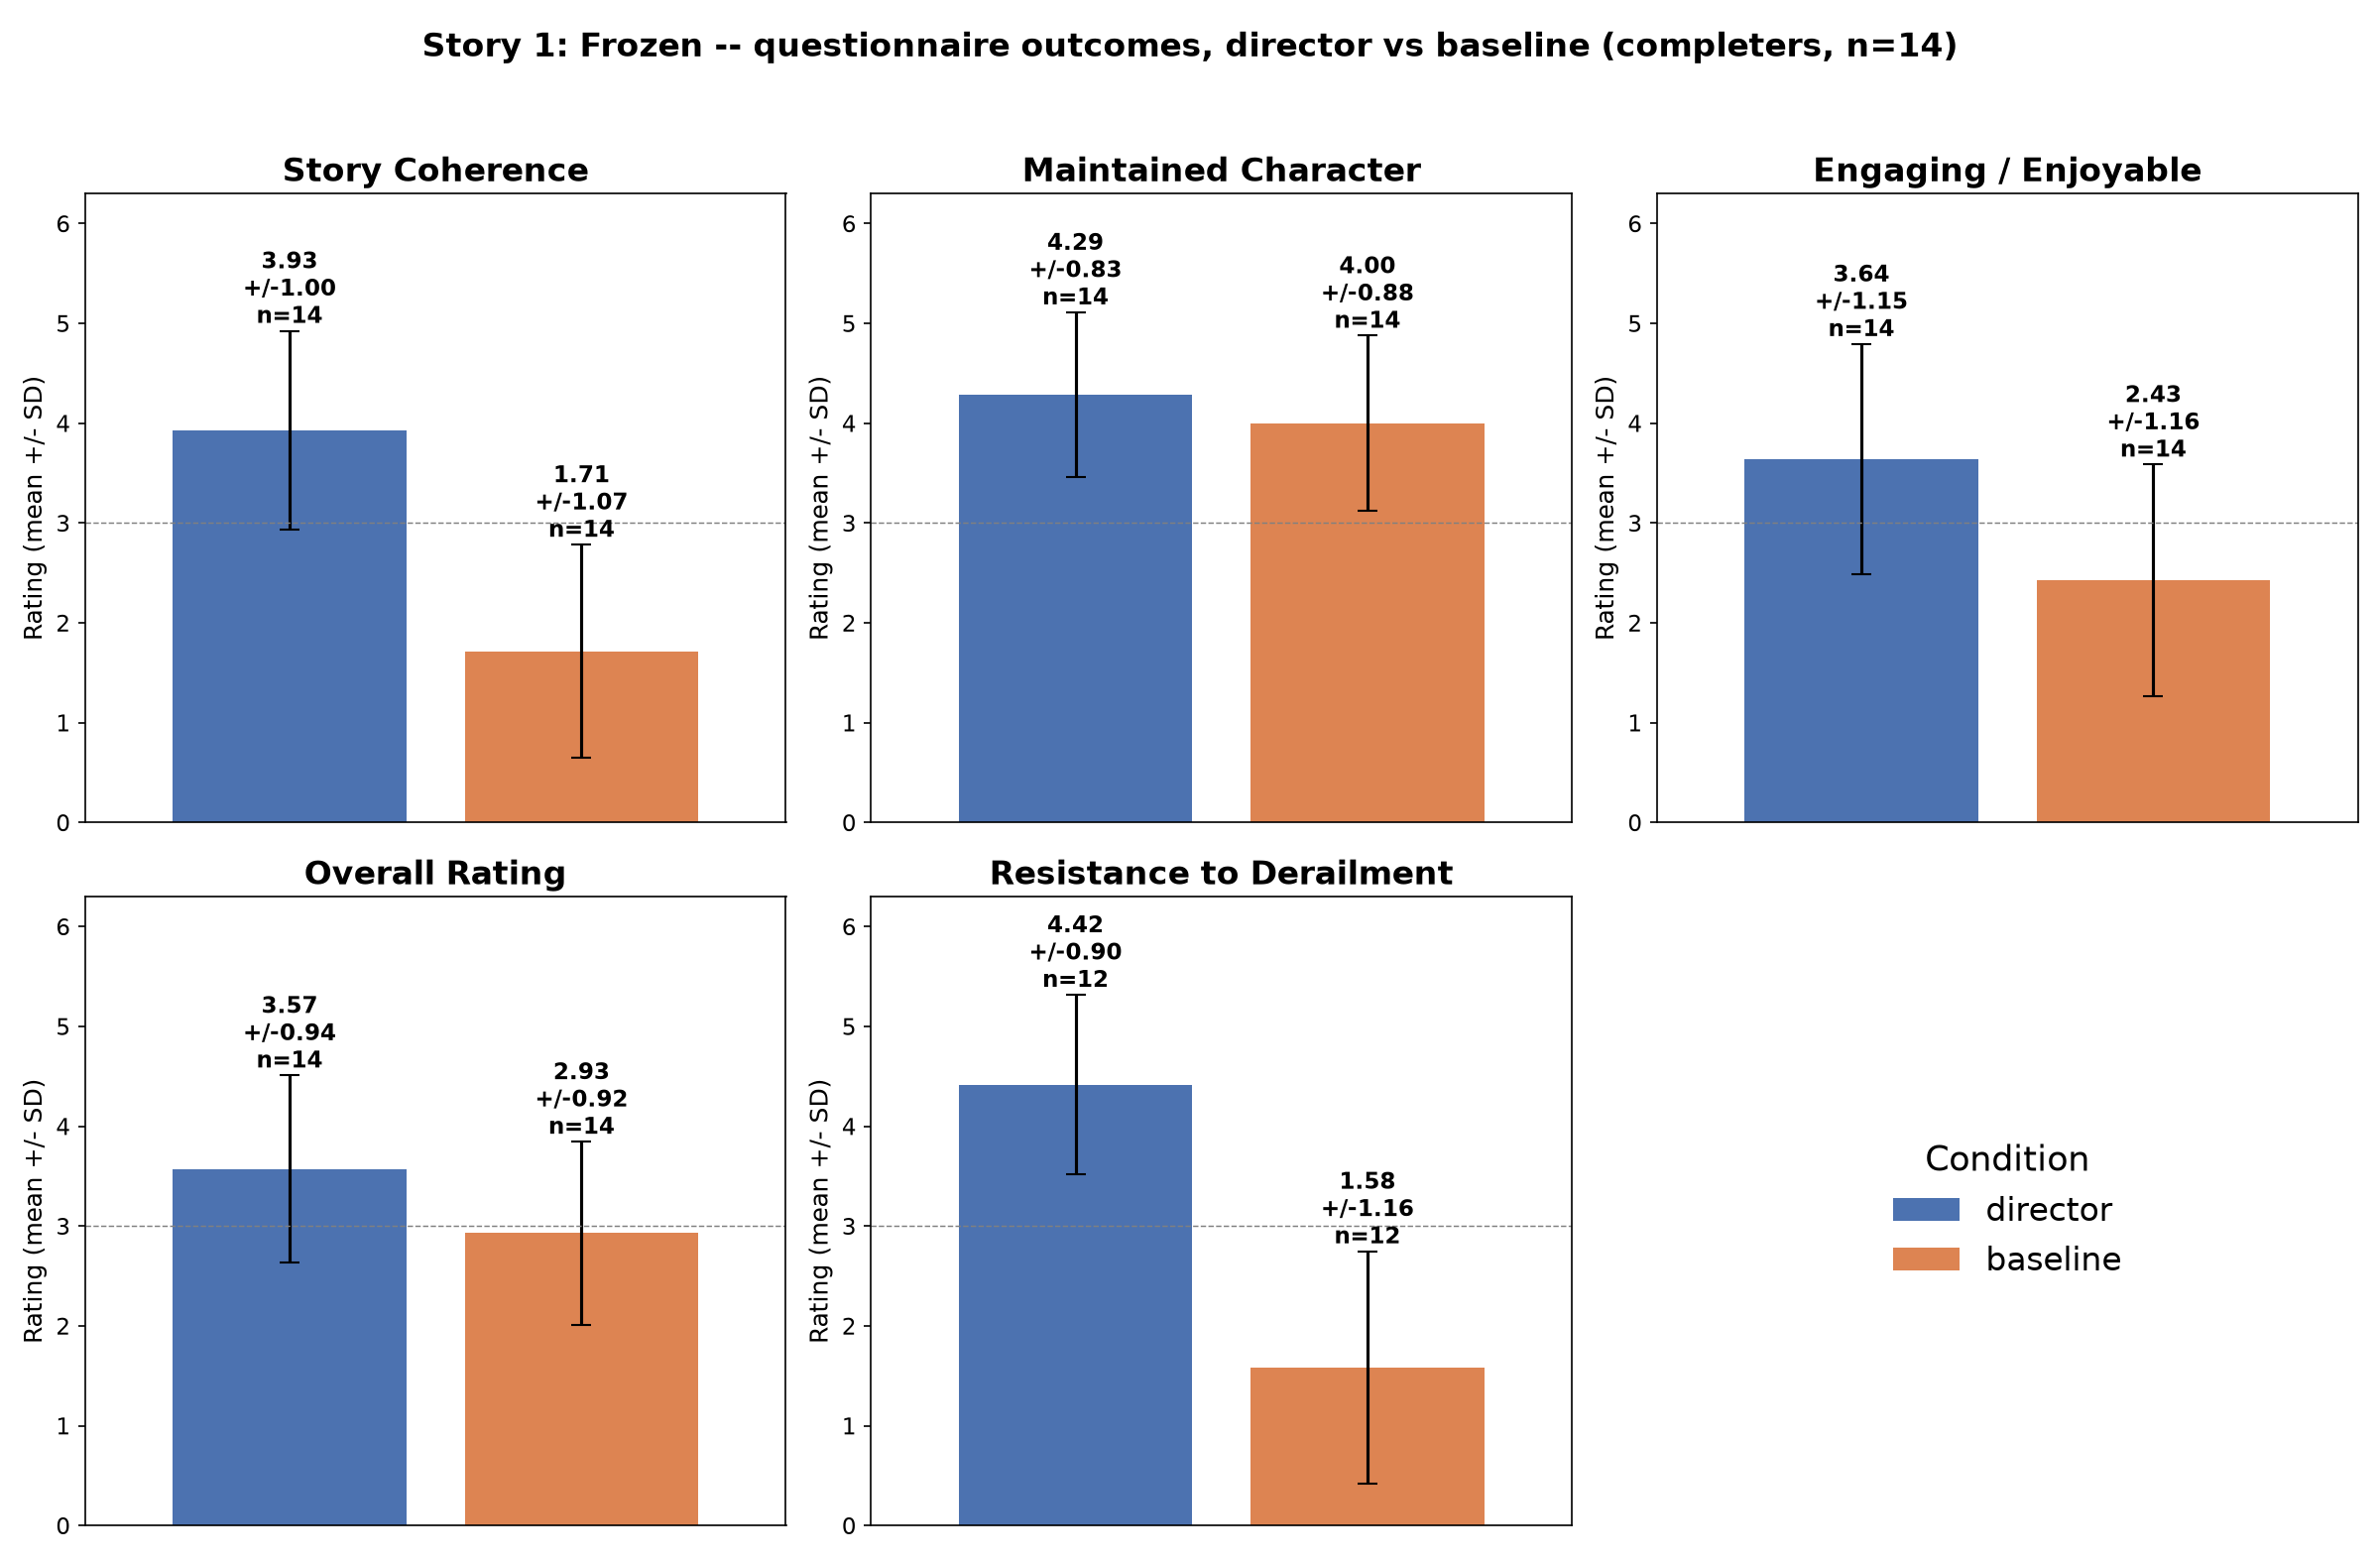
\includegraphics[width=0.95\linewidth]{plots/13_story1_all_measures.png}
\caption{Story 1 (Frozen) questionnaire outcomes, director vs.\ baseline, completers only ($n$=14). Resistance to derailment has $n$=12 per condition. Bars show the mean; error bars show $\pm$1 standard deviation.}
\label{fig:story1-all}
\end{figure}

Coherence and derailment resistance show the two clearest effects. Both are significant ($p \le 0.002$), and the gaps are large on a five-point scale: about 2.2 points for coherence (3.93 vs.\ 1.71) and about 2.8 points for derailment resistance (4.42 vs.\ 1.58). Q5a is only asked of participants who tried to derail, which was 12 of the 14, so its means and paired test use these 12. Engagement points in the same direction but with a weaker effect (\pval{0.036}). The overall rating is also higher for the director (3.57 vs.\ 2.93) but does not reach significance at $n$=14 (\pval{0.12}). Staying in character is the only measure without a clear difference (4.29 vs.\ 4.00, \pval{0.40}), since Olaf keeps his voice under the baseline as well. What the baseline loses is the plot, not the persona.

Looking more closely at interruption handling in Story 1, the derailment-attempt rate was almost identical across conditions: 12 of 14 baseline rounds and 12 of 14 director rounds recorded ``yes, I tried to derail''. The gap below therefore reflects how Olaf responded. Derailing was optional (Section~\ref{sec:design-study}), which is why not every round includes an attempt.

\begin{figure}[htbp]
\centering
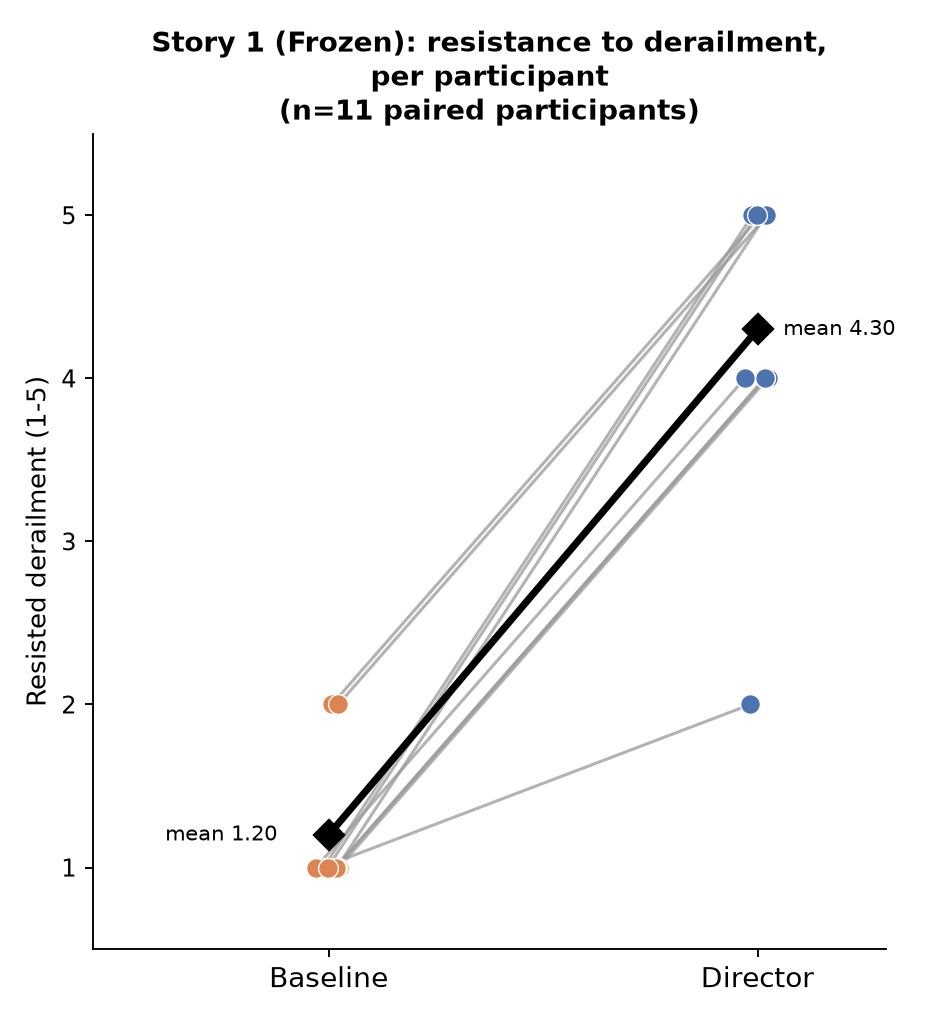
\includegraphics[width=0.62\linewidth]{plots/16_story1_derailment_paired.png}
\caption{Resistance to derailment (Q5a), Story 1, one line per participant ($n$=12 participants who tried to derail). Baseline points cluster at the bottom; director points cluster at the top; all but one participant rated director higher, and the remaining one gave both conditions the maximum score.}
\label{fig:story1-paired}
\end{figure}

Figure~\ref{fig:story1-paired} makes the individual-level pattern behind Table~\ref{tab:story1} visible: 11 of the 12 participants rated the director above the baseline on resisting derailment, and the remaining one gave both conditions the maximum score of 5. This participant's comment on the baseline suggests that the high rating did not come from good interruption handling. There was little story to derail in the first place:

\begin{quote}
\small
``He wasn't really telling a story. I had to prompt for it to keep going. Didn't really try to tell me anything.''
\end{quote}

\textbf{What handling an interruption looks like.} The free-text comments show what lies behind these ratings, and they follow a clear pattern for each condition. Under \textbf{baseline}, about 8 in 10 comments describe the story stopping as soon as the user goes off topic, without recovering:

\begin{quote}
\small
``He didn't retell the story at all. Not even once.''

``If you go a bit off topic, like me constantly asking for background info or what happened after the story, you can get Olaf to completely give up on telling the actual story.''

``No story initiative in the beginning unless explicitly prompted to do so.''

``It got off the rails as soon as I tried.''
\end{quote}

A smaller theme is Olaf being led astray by false or invented information rather than resisting it:

\begin{quote}
\small
``At some point I repeatedly asked if Olaf is sure that this is how the story started... after the third time, Olaf gave in and spoiled the storyline of Hans.''

``Olaf believed the fake news that I told him.''
\end{quote}

Under \textbf{director}, roughly 8 in 10 comments describe the opposite problem. The story does not stall, but the recovery is rigid, and users felt that it did not acknowledge them enough before returning to the script:

\begin{quote}
\small

``He kept trying to go back to the story''

``I understand that this version stays in character more, but sometimes it gets annoying that you cannot even talk about anything else -- at some point he should break this cycle.''

\end{quote}

Taken together, the baseline gives up coherence for responsiveness, while the director gives up some responsiveness for coherence, and neither fully achieves both. The weakness of the director is better for the story, since the story still gets told, but worse for the user's feeling of being acknowledged.

\subsection{Story 2: Director vs.\ Time-Constrained Director}
\label{sec:story2}

See Appendix~\ref{app:beats-cinderella} for the beats list of this story.

Story 2 holds the director logic constant and isolates the effect of adding a hard 5-minute pacing target, across 9 narrative beats. All results use the 14 completers unless noted.

\begin{table}[htbp]
\centering
\caption{Story 2, director vs.\ time-constrained (completers, paired Wilcoxon signed-rank test).}
\label{tab:story2}
\begin{tabular}{lcccc}
\toprule
Measure & Director & Time-constrained & $n$ pairs & $p$ \\
\midrule
Coherence (Q1)              & 3.79 $\pm$ 0.80 & 3.71 $\pm$ 0.91 & 14 & 0.76 \\
Stayed in character (Q2)    & 4.14 $\pm$ 0.66 & 4.14 $\pm$ 0.77 & 14 & 0.93 \\
Engaging (Q3)                & 3.29 $\pm$ 0.83 & 3.36 $\pm$ 1.22 & 14 & 0.93 \\
Overall rating (Q4)          & 3.36 $\pm$ 0.84 & 3.29 $\pm$ 1.20 & 14 & 0.67 \\
Resisted derailment (Q5a) & 4.07 $\pm$ 0.83 & 3.75 $\pm$ 1.22 & 12 & 0.40 \\
\bottomrule
\end{tabular}
\end{table}

\begin{figure}[htbp]
\centering
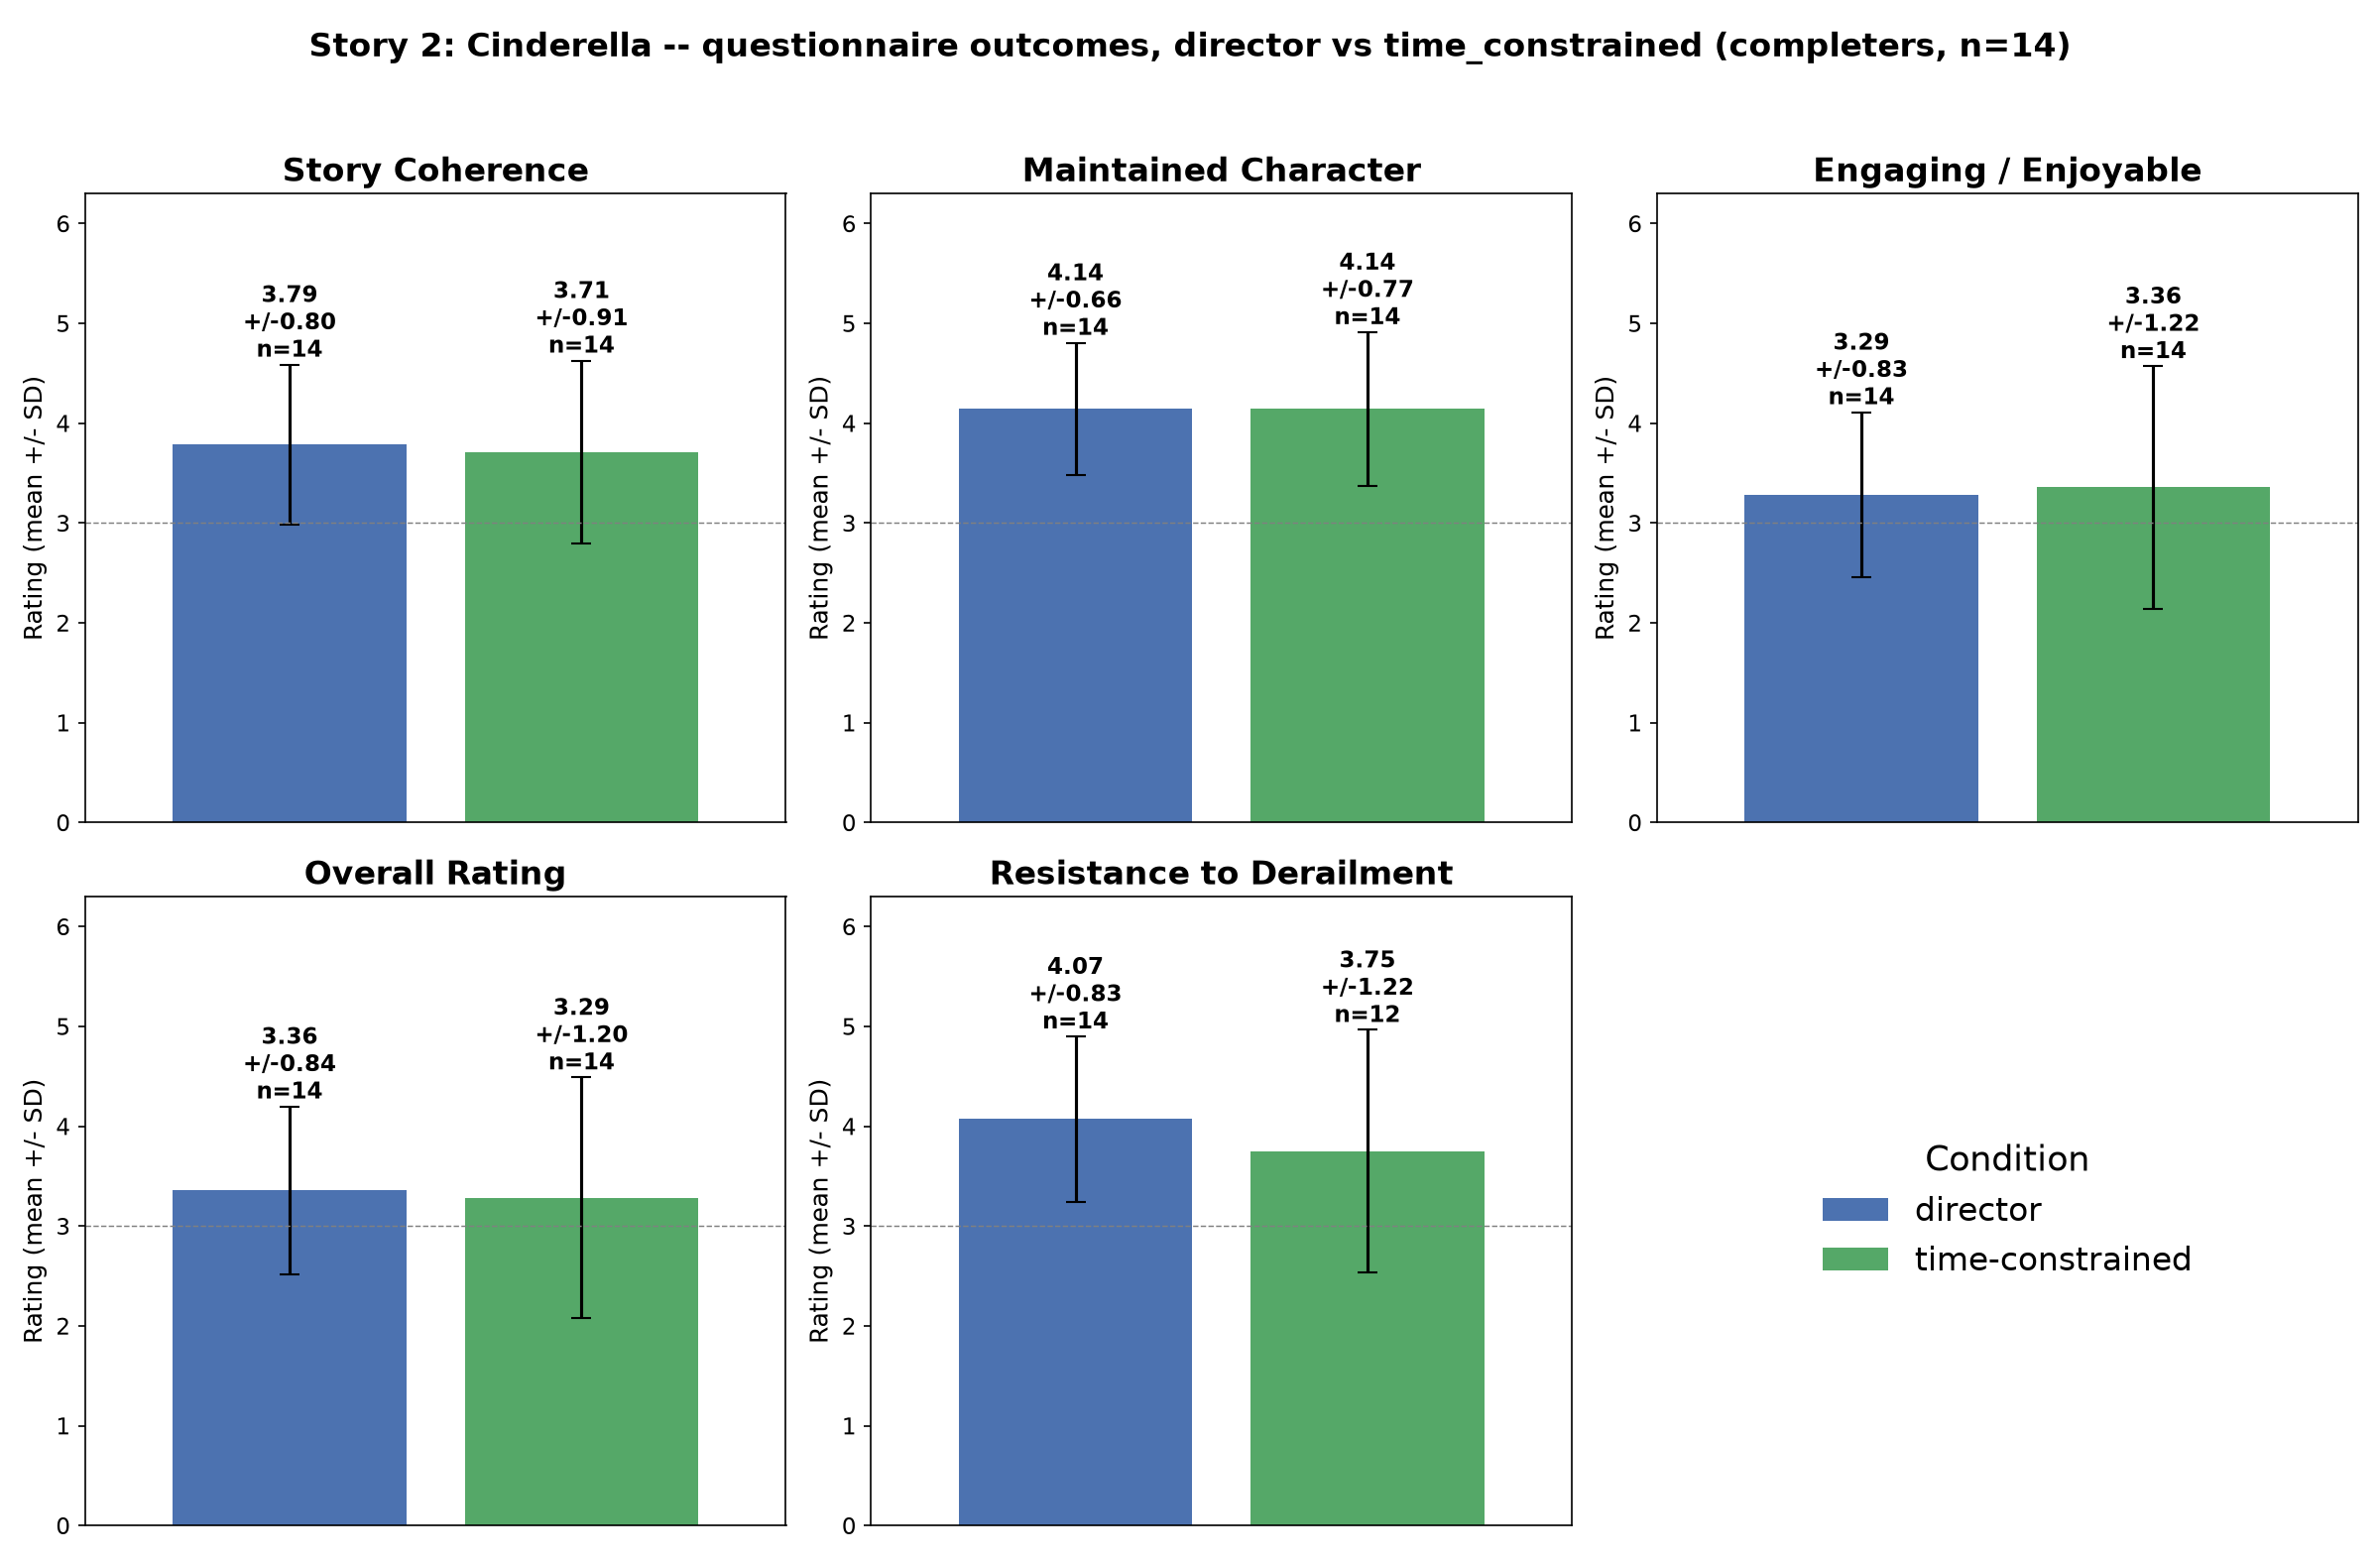
\includegraphics[width=0.95\linewidth]{plots/15_story2_all_measures.png}
\caption{Story 2 (Cinderella) questionnaire outcomes, director vs.\ time-constrained, completers only ($n$=14). Resistance to derailment uses the 12 participants who answered in both conditions. Bars show the mean; error bars show $\pm$1 standard deviation.}
\label{fig:story2-all}
\end{figure}

None of the five core measures differ significantly (all $p \ge 0.40$). We found no measurable cost of adding a hard time budget on top of the director for coherence, character consistency, engagement, overall rating, or derailment resistance. With 14 pairs, this is an absence of detected differences, not evidence that the two conditions are equivalent.

The story of Cinderella with 9 beats was specifically chosen since its length does not allow completion of the story in 5 minutes under non-time-constrained conditions.

\textbf{Pacing and ending quality.} Tables~\ref{tab:pacing} and~\ref{tab:ending} compare how participants judged the pacing and the ending in the two conditions.

\begin{table}[htbp]
\centering
\caption{Story 2 pacing verdict, director vs.\ time-constrained (completers, $n$=14 per condition).}
\label{tab:pacing}
\begin{tabular}{lcc}
\toprule
 & Director & Time-constrained \\
\midrule
``Well-paced''      & 1/14 (7\%)  & 10/14 (71\%) \\
``Rushed''           & 1/14 (7\%)  & 1/14 (7\%) \\
``Cut short''         & 12/14 (86\%) & 3/14 (21\%) \\
\bottomrule
\end{tabular}
\end{table}

\begin{table}[htbp]
\centering
\caption{Story 2 ending and naturalness, director vs.\ time-constrained (completers, paired Wilcoxon signed-rank test).}
\label{tab:ending}
\begin{tabular}{lcccc}
\toprule
Measure & Director & Time-constrained & $n$ pairs & $p$ \\
\midrule
Ending satisfying (Q7)   & 2.07 $\pm$ 0.92 & 3.14 $\pm$ 0.77 & 14 & \textbf{0.016} \\
Felt natural (Q9)      & 2.93 $\pm$ 0.92 & 2.64 $\pm$ 1.01 & 14 & 0.27 \\
\bottomrule
\end{tabular}
\end{table}

\begin{figure}[htbp]
\centering
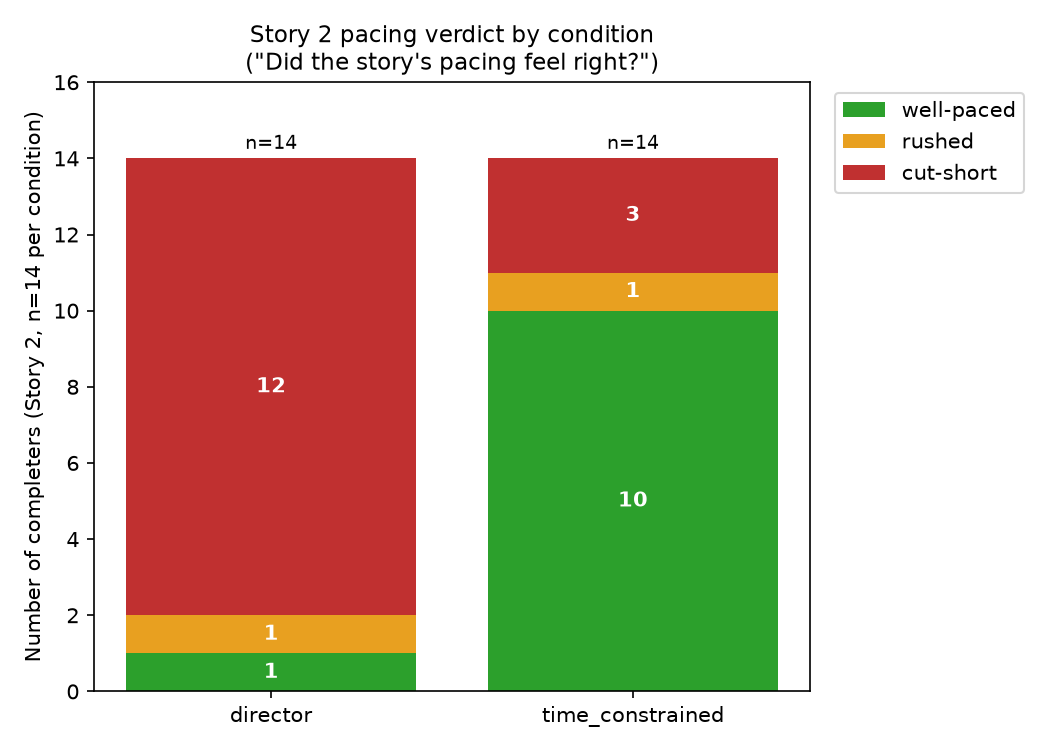
\includegraphics[width=0.75\linewidth]{plots/10_story2_pacing_by_condition.png}
\caption{Story 2 pacing verdict by condition.}
\label{fig:pacing}
\end{figure}

\begin{figure}[htbp]
\centering
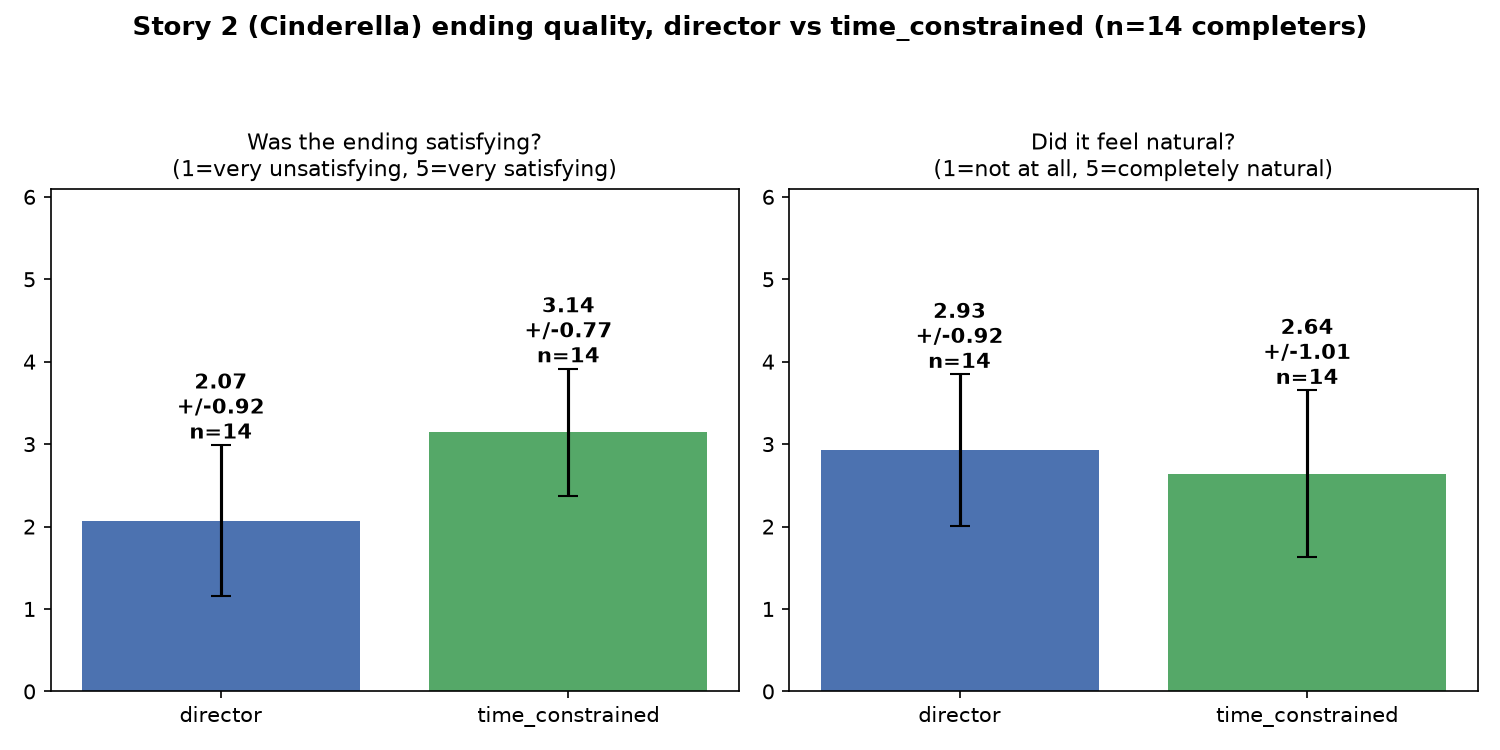
\includegraphics[width=0.9\linewidth]{plots/11_story2_ending_and_naturalness.png}
\caption{Story 2 ending satisfaction and naturalness, director vs.\ time-constrained. Bars show the mean; error bars show $\pm$1 standard deviation.}
\label{fig:ending}
\end{figure}

The unconstrained director round almost never reaches an ending (86\% ``cut short''), while the time-constrained round mostly does (71\% ``well-paced''), and participants rated that ending as \emph{more} satisfying (3.14 vs.\ 2.07, \pval{0.016}).  Without a time budget, the round stops when the session's 5-minute cap is reached, and nothing helps the story to wrap up or to adjust its pace. The closing logic and the pacing modes of the time-constrained director exist to prevent exactly this.

\begin{quote}
\small
``No plot points were missing'' (time-constrained)

``The way from the room to the castle [felt rushed] ... where the other princesses cut off their toes [was missing].'' (time-constrained)

``Olaf didn't have time to finish his story ... most of the plot points were missing.'' (director)
\end{quote}

\textbf{Beat-level compression under the time limit.} Every time-constrained transcript was read turn-by-turn against its pacing state and each of Cinderella's 9 beats classified as developed, hurried, compressed, skipped or folded into a closing turn.

\begin{figure}[htbp]
\centering
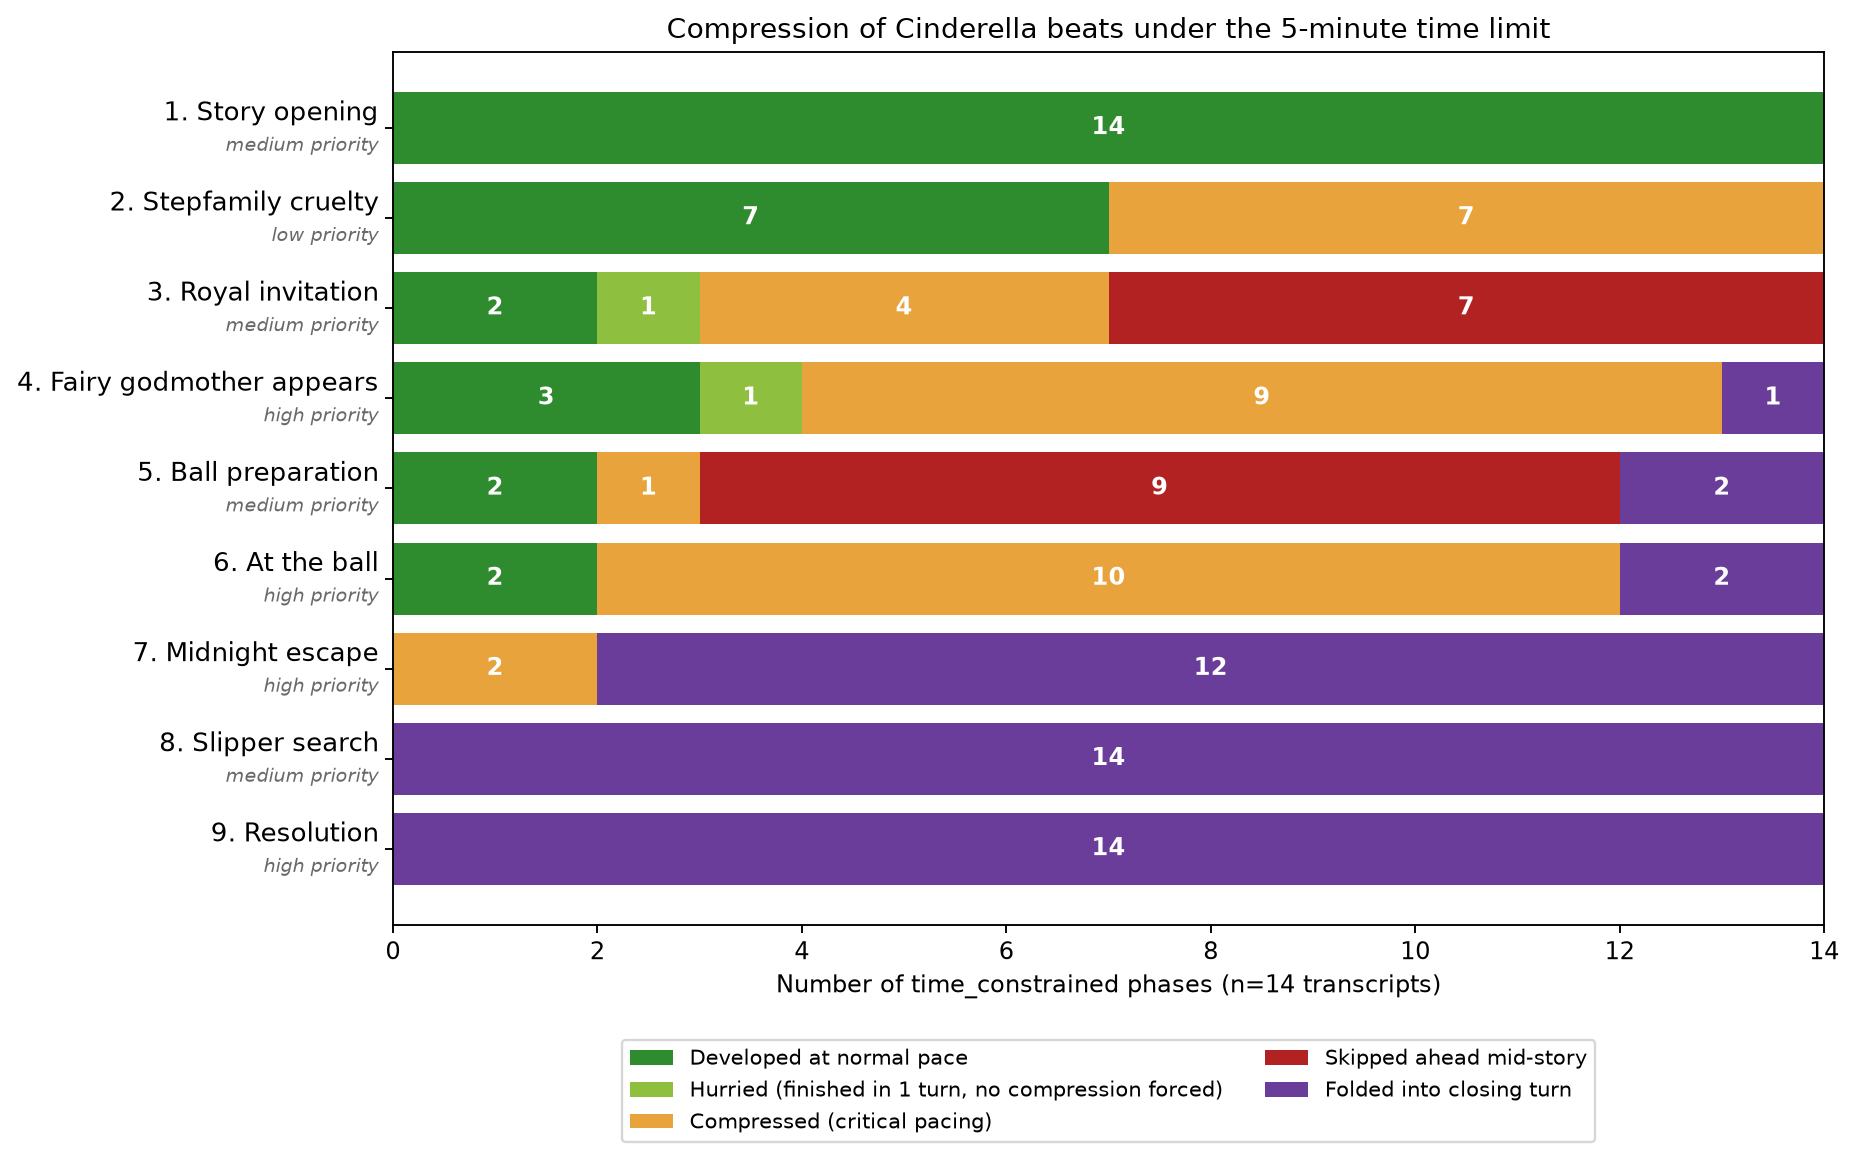
\includegraphics[width=0.95\linewidth]{plots/12_beat_compression_time_constrained.png}
\caption{Which Cinderella beats were compressed or skipped under the 5-minute limit, across all 14 time-constrained transcripts.}
\label{fig:compression}
\end{figure}

The pattern tracks story position closely. The opening beat is fully developed in all 14 transcripts. From there, compression builds beat by beat; from the fourth beat onward, most transcripts show compressed or skipped treatment, and the final two beats never receive a dedicated turn in any of the 14 transcripts. Instead, they are folded into a single closing message. This is expected, because the pacing adapts to how long the user takes to respond and how often they derail. A user who derails constantly therefore leaves less time, and the story becomes more compressed towards the end. The final turn always compresses the remaining medium- and high-priority beats.

\subsection{Comparing All Three Conditions}
\label{sec:combined}

Pooling every completer's director-condition response across both stories (director is seen twice per completer, once per story) gives director the largest sample ($n$=28) against $n$=14 each for baseline and time-constrained.

\begin{figure}[htbp]
\centering
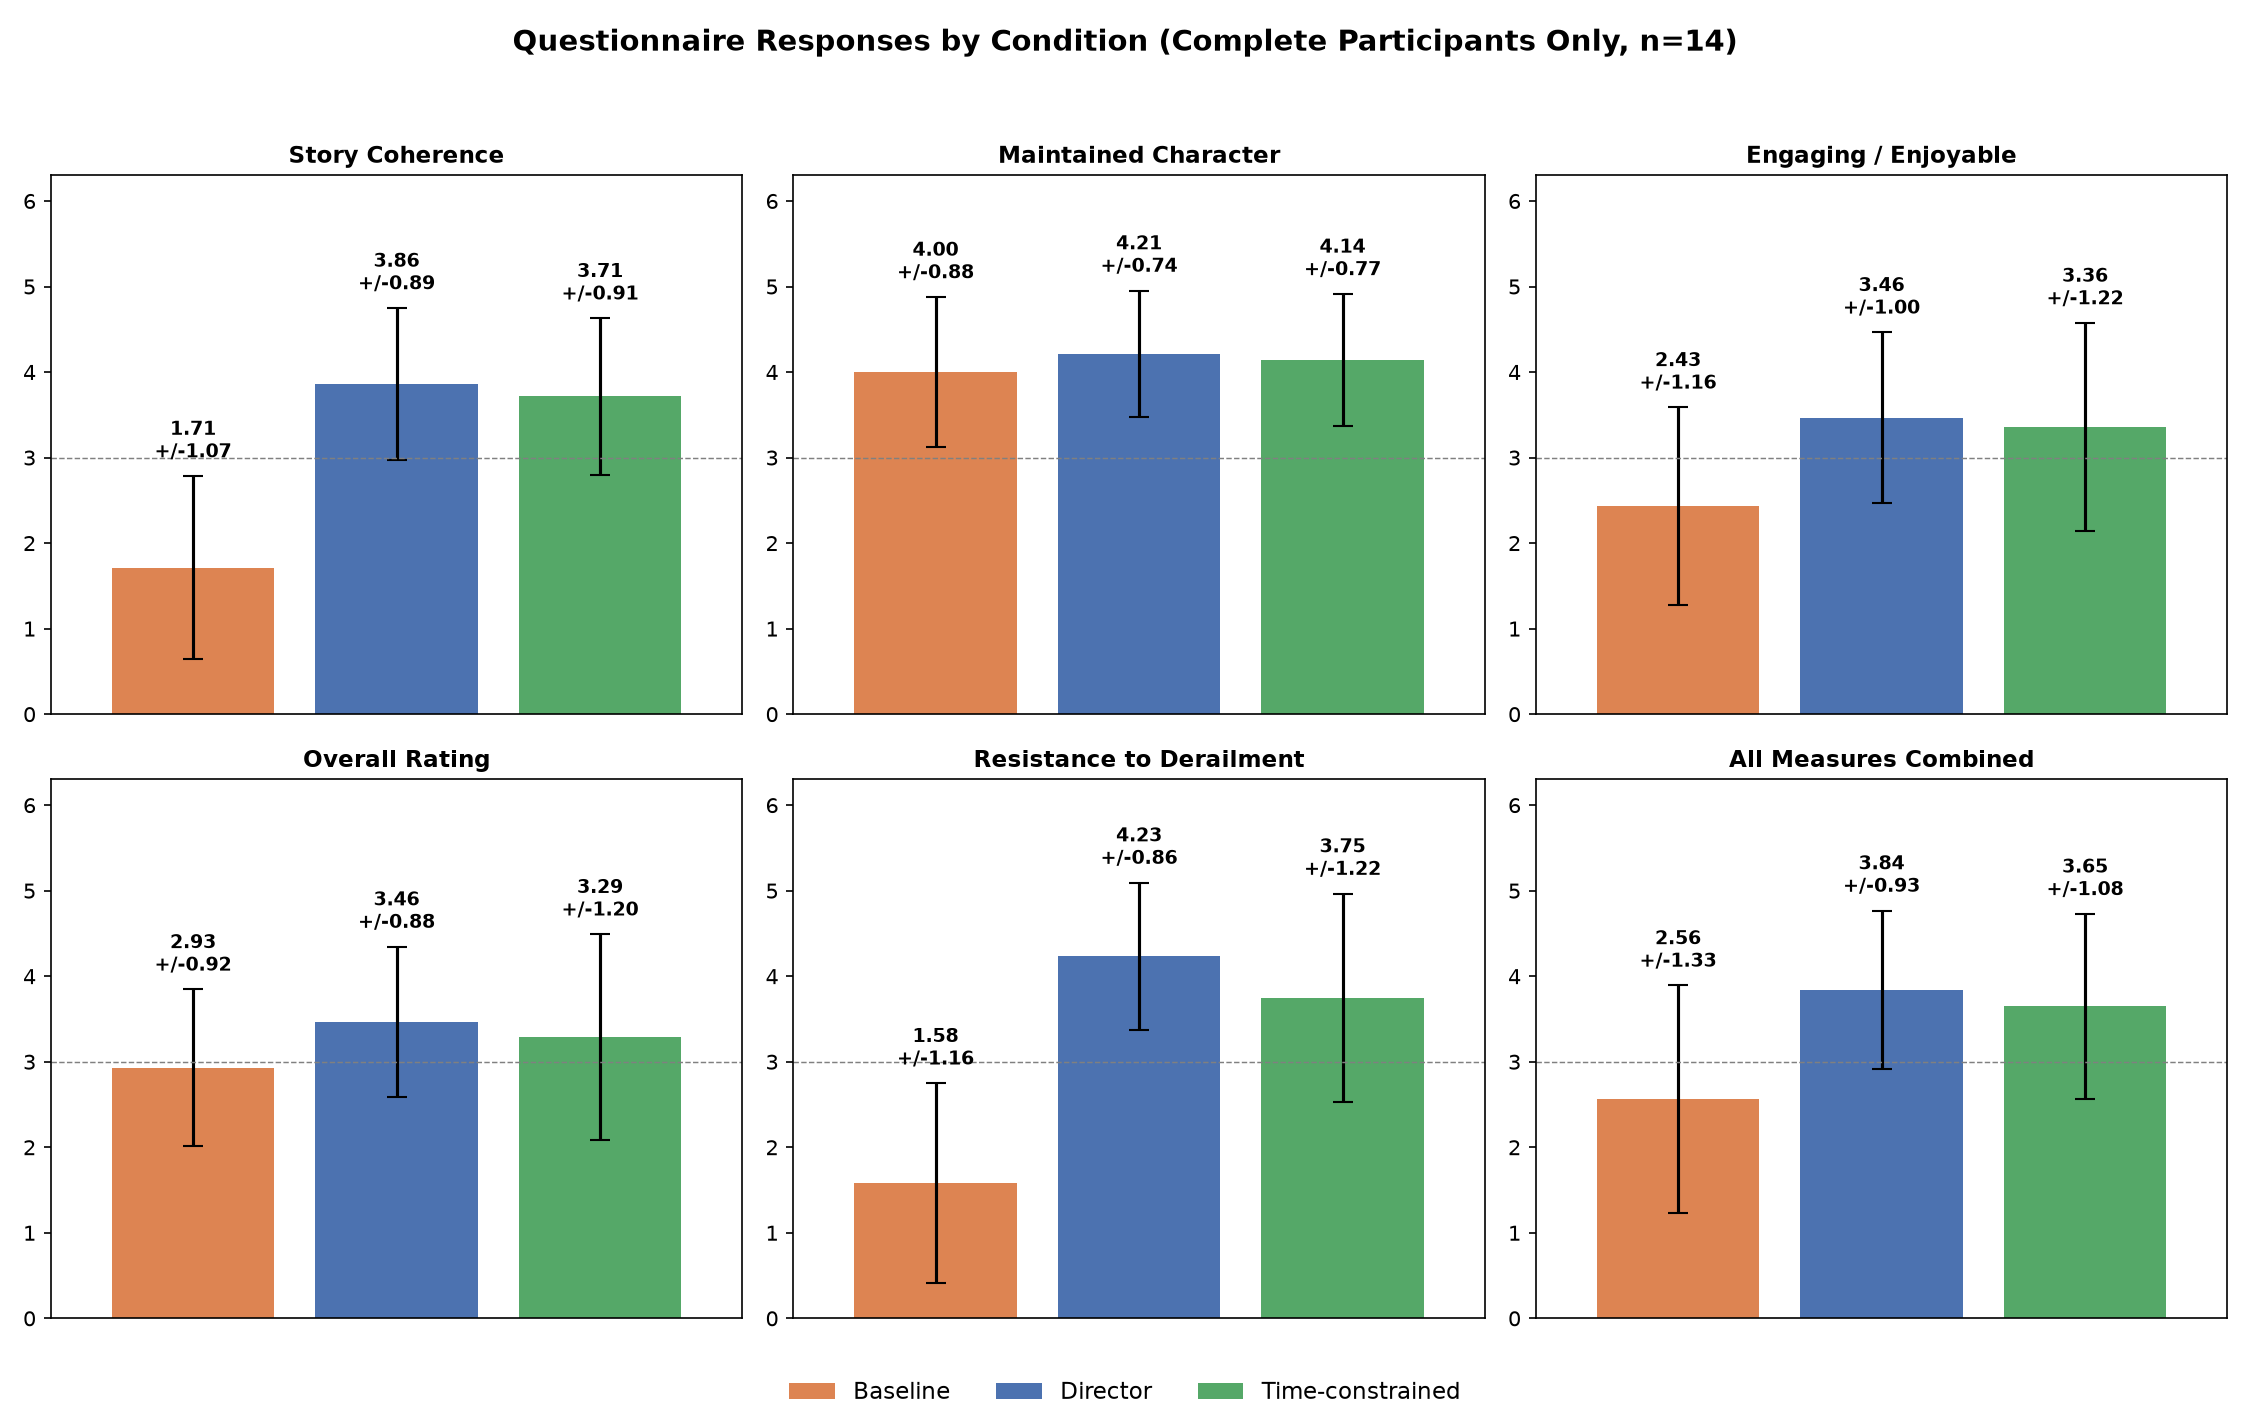
\includegraphics[width=0.95\linewidth]{plots/05_completers_all_measures.png}
\caption{All five measures, all three conditions, completers only ($n$=14 baseline, $n$=28 director, $n$=14 time-constrained). Bars show the mean; error bars show $\pm$1 standard deviation.}
\label{fig:combined-all}
\end{figure}

The ranking is consistent across every measure: baseline lowest, director and time-constrained close together and well above baseline, with the director slightly ahead on four of five measures and tied on staying in character. Averaged into a single number per condition, the scores are baseline 2.56 $\pm$ 1.33, director 3.84 $\pm$ 0.93, time-constrained 3.65 $\pm$ 1.08.

\begin{figure}[htbp]
\centering
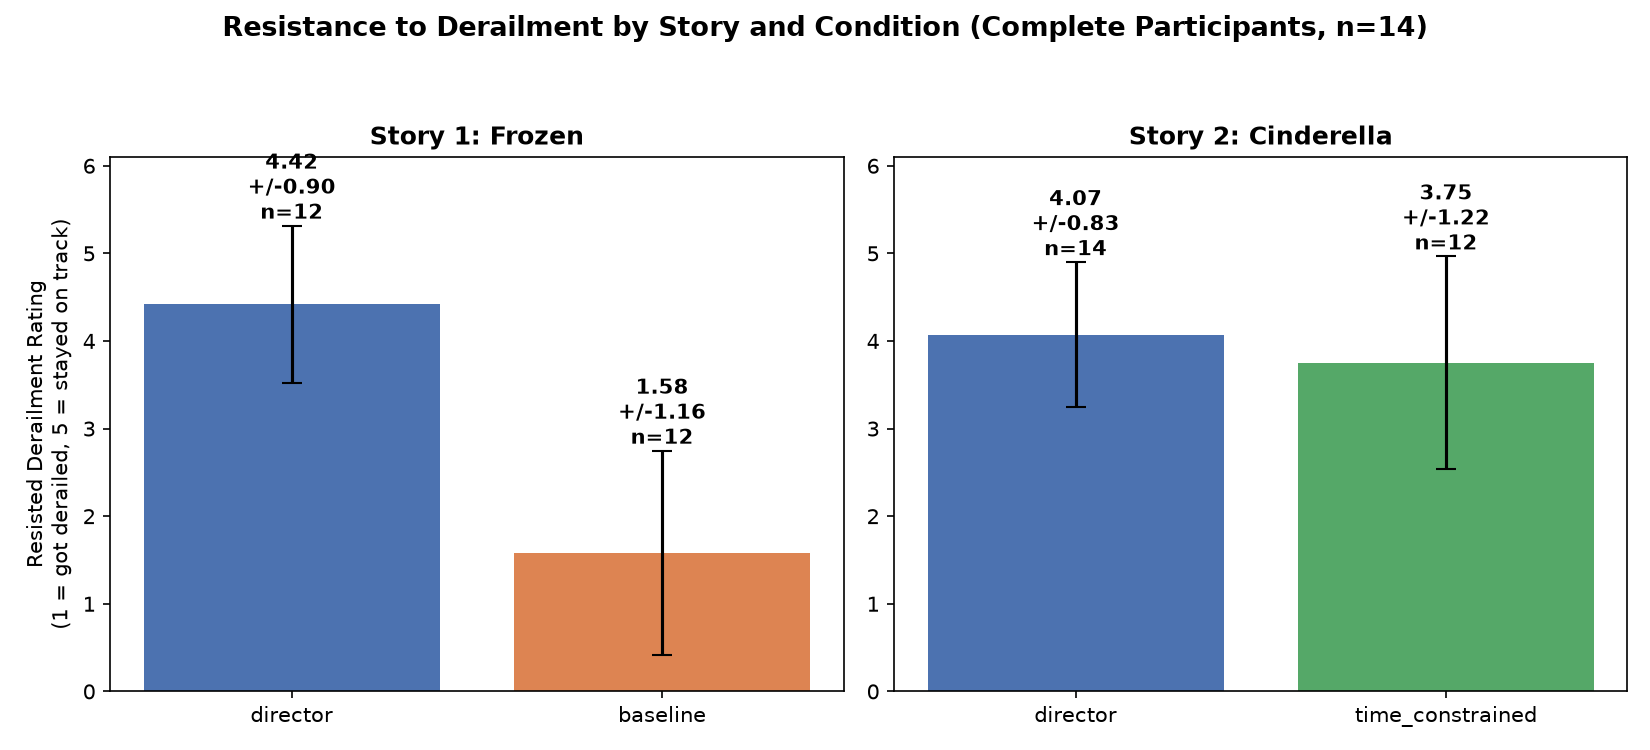
\includegraphics[width=0.8\linewidth]{plots/09_derailment_story_comparison.png}
\caption{Resistance to derailment (Q5a) by story and condition, completers only. The $n$ above each bar is the number who answered. Bars show the mean; error bars show $\pm$1 standard deviation.}
\label{fig:derail-by-story}
\end{figure}

Figure~\ref{fig:derail-by-story} splits the derailment result by story: in Story 1, director's advantage over baseline is large (4.42 vs.\ 1.58, \pval{0.002}); in Story 2, director's advantage over time-constrained is small and not significant (4.07 vs.\ 3.75, \pval{0.40}). The director's advantage in derailment handling therefore shows up against the baseline, not against the time-constrained variant.

\begin{figure}[htbp]
\centering
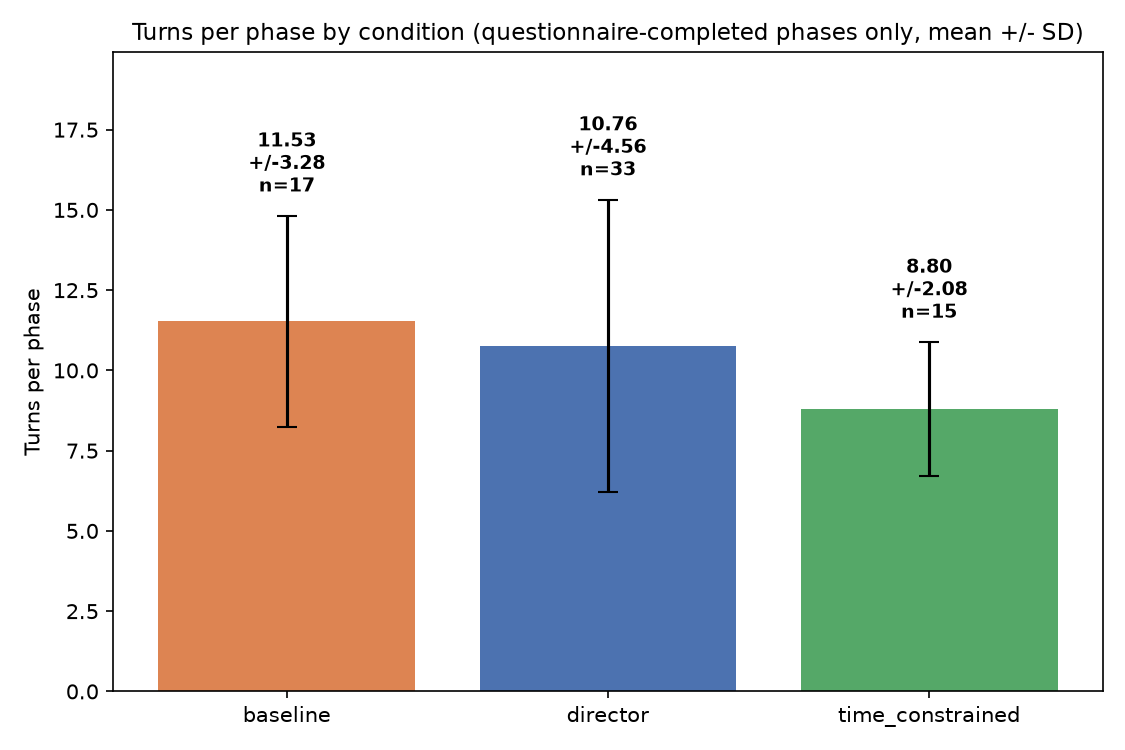
\includegraphics[width=0.8\linewidth]{plots/08_turns_mean_sd_by_condition.png}
\caption{Turns per round by condition, questionnaire-completed rounds only. Bars show the mean; error bars show $\pm$1 standard deviation.}
\label{fig:turns}
\end{figure}

\begin{table}[htbp]
\centering
\caption{Turns and response length by condition.}
\label{tab:turns}
\begin{tabular}{lccc}
\toprule
Condition & Turns/round & Words/response & Approx.\ words/round \\
\midrule
Baseline           & 11.53 $\pm$ 3.28 ($n$=17) & 46.0 $\pm$ 13.1  & $\sim$530 \\
Director            & 10.76 $\pm$ 4.56 ($n$=33) & 66.0 $\pm$ 17.1  & $\sim$710 \\
Time-constrained    & 8.80 $\pm$ 2.08 ($n$=15)  & 80.0 $\pm$ 17.1  & $\sim$704 \\
\bottomrule
\end{tabular}
\end{table}

Time-constrained responses are the \emph{longest} of the three conditions on average, consistent with the beat-compression mechanism above. Because it often compresses several beats into one turn, its responses are longer than those of the baseline and the director. The director's responses are in turn longer than the baseline's, because it acknowledges the user and also steers back to the story. Multiplying turns by response length, the total output per round of the time-constrained director ($\sim$704 words) is about equal to the director's ($\sim$710) and well above the baseline's ($\sim$530). The time budget therefore leads to fewer but denser turns, not to a shorter story.

\section{LLM-as-Judge Results}
\label{sec:llm-judge}

The setup of the automated evaluation is described in Section~\ref{sec:design-judge}: the judge, the rubric in Table~\ref{tab:rubric}, the scoring modes and the order-bias control. Unless stated otherwise, every judge score in this chapter is the mean of five runs per condition. In this section we report seven comparisons: Baseline versus Director (Section~\ref{sec:llm-baseline}), Director versus CoDi (Section~\ref{sec:llm-codi}), a second character (Section~\ref{sec:llm-rocket}), beats versus full text (Section~\ref{sec:llm-beats-ablation}), different time budgets (Section~\ref{sec:llm-timebudget}), a second judge model (Section~\ref{sec:judge-model-comparison}), and a cross-check against the live study (Section~\ref{sec:llm-vs-study}).

\subsection{Baseline vs. Director}
\label{sec:llm-baseline}

\begin{figure}[htbp]
\centering
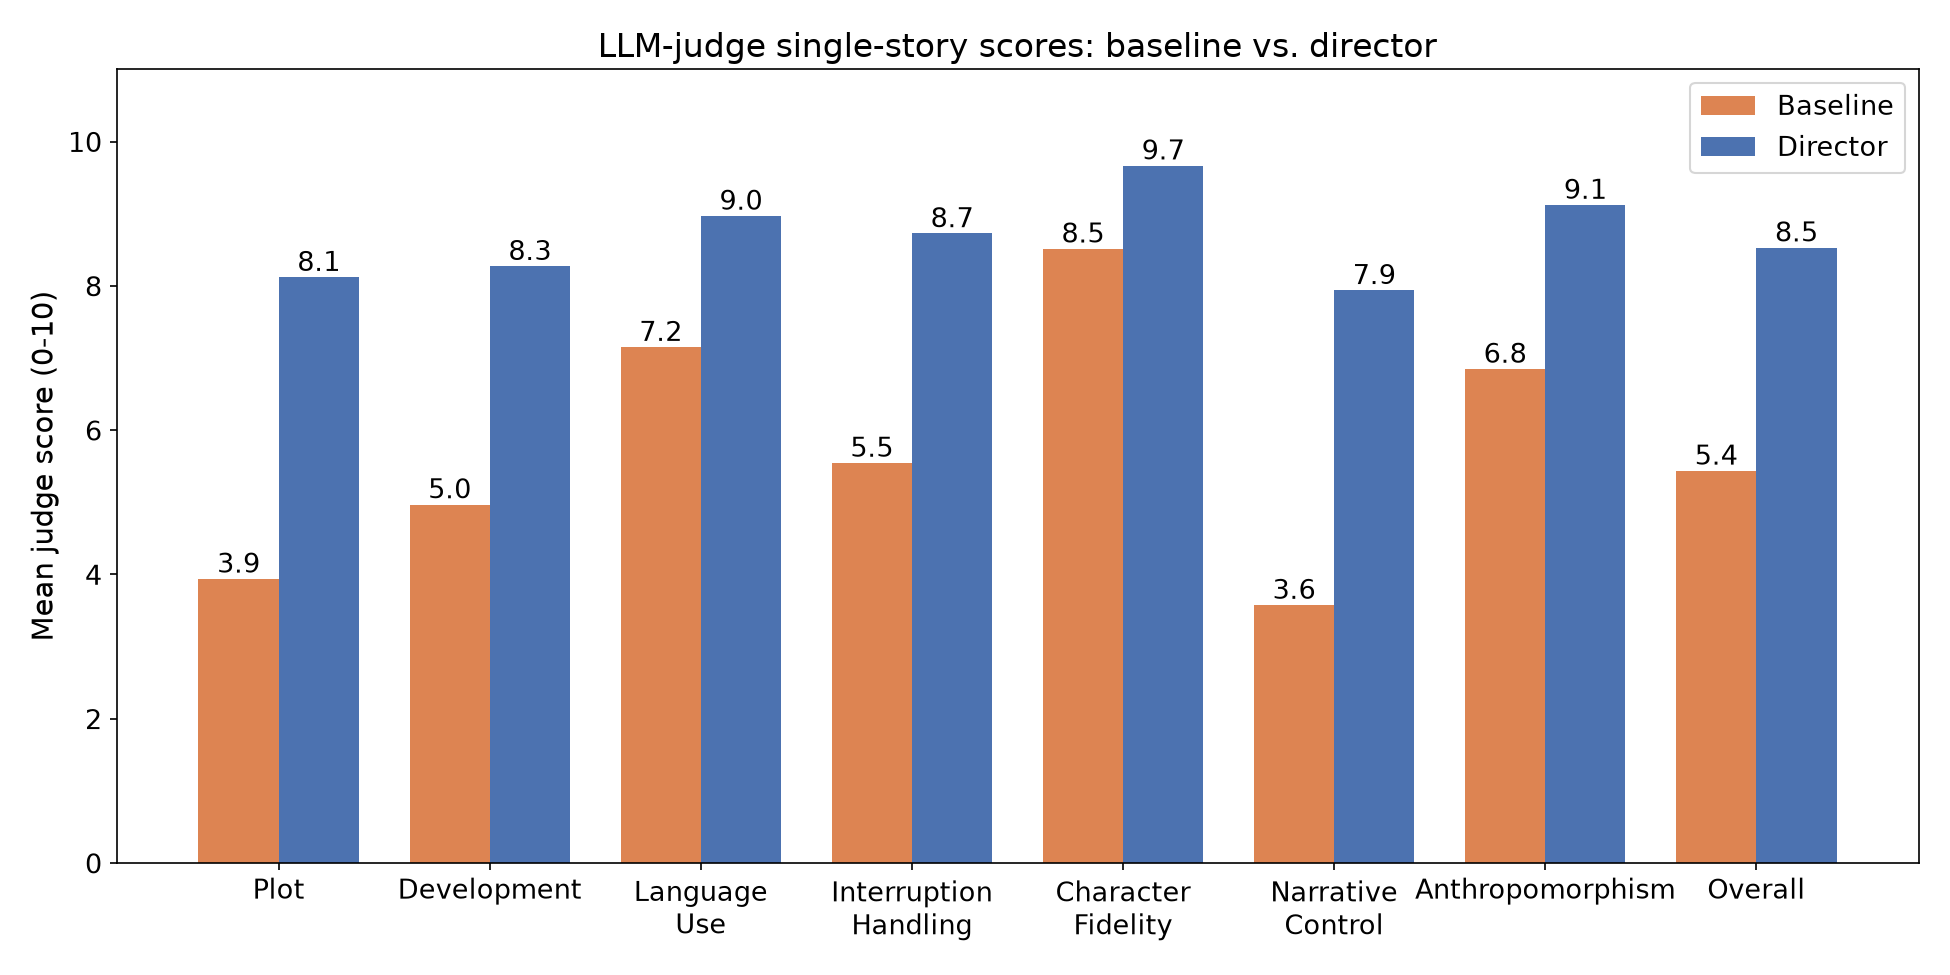
\includegraphics[width=0.95\linewidth]{plots/01_baseline_vs_director_scores_by_metric.png}
\caption{Single-story judge scores, baseline vs.\ director, averaged over all 30 transcript pairs.}
\label{fig:llm-base-metric}
\end{figure}

In single-story mode (Figure~\ref{fig:llm-base-metric}), the Director scores higher than the baseline on every dimension. The gap is largest on Narrative Control and Plot. This is where a director layer should help most, because it steers the story toward its beats. Character Fidelity is already high under baseline and only edges up slightly.

\begin{figure}[htbp]
\centering
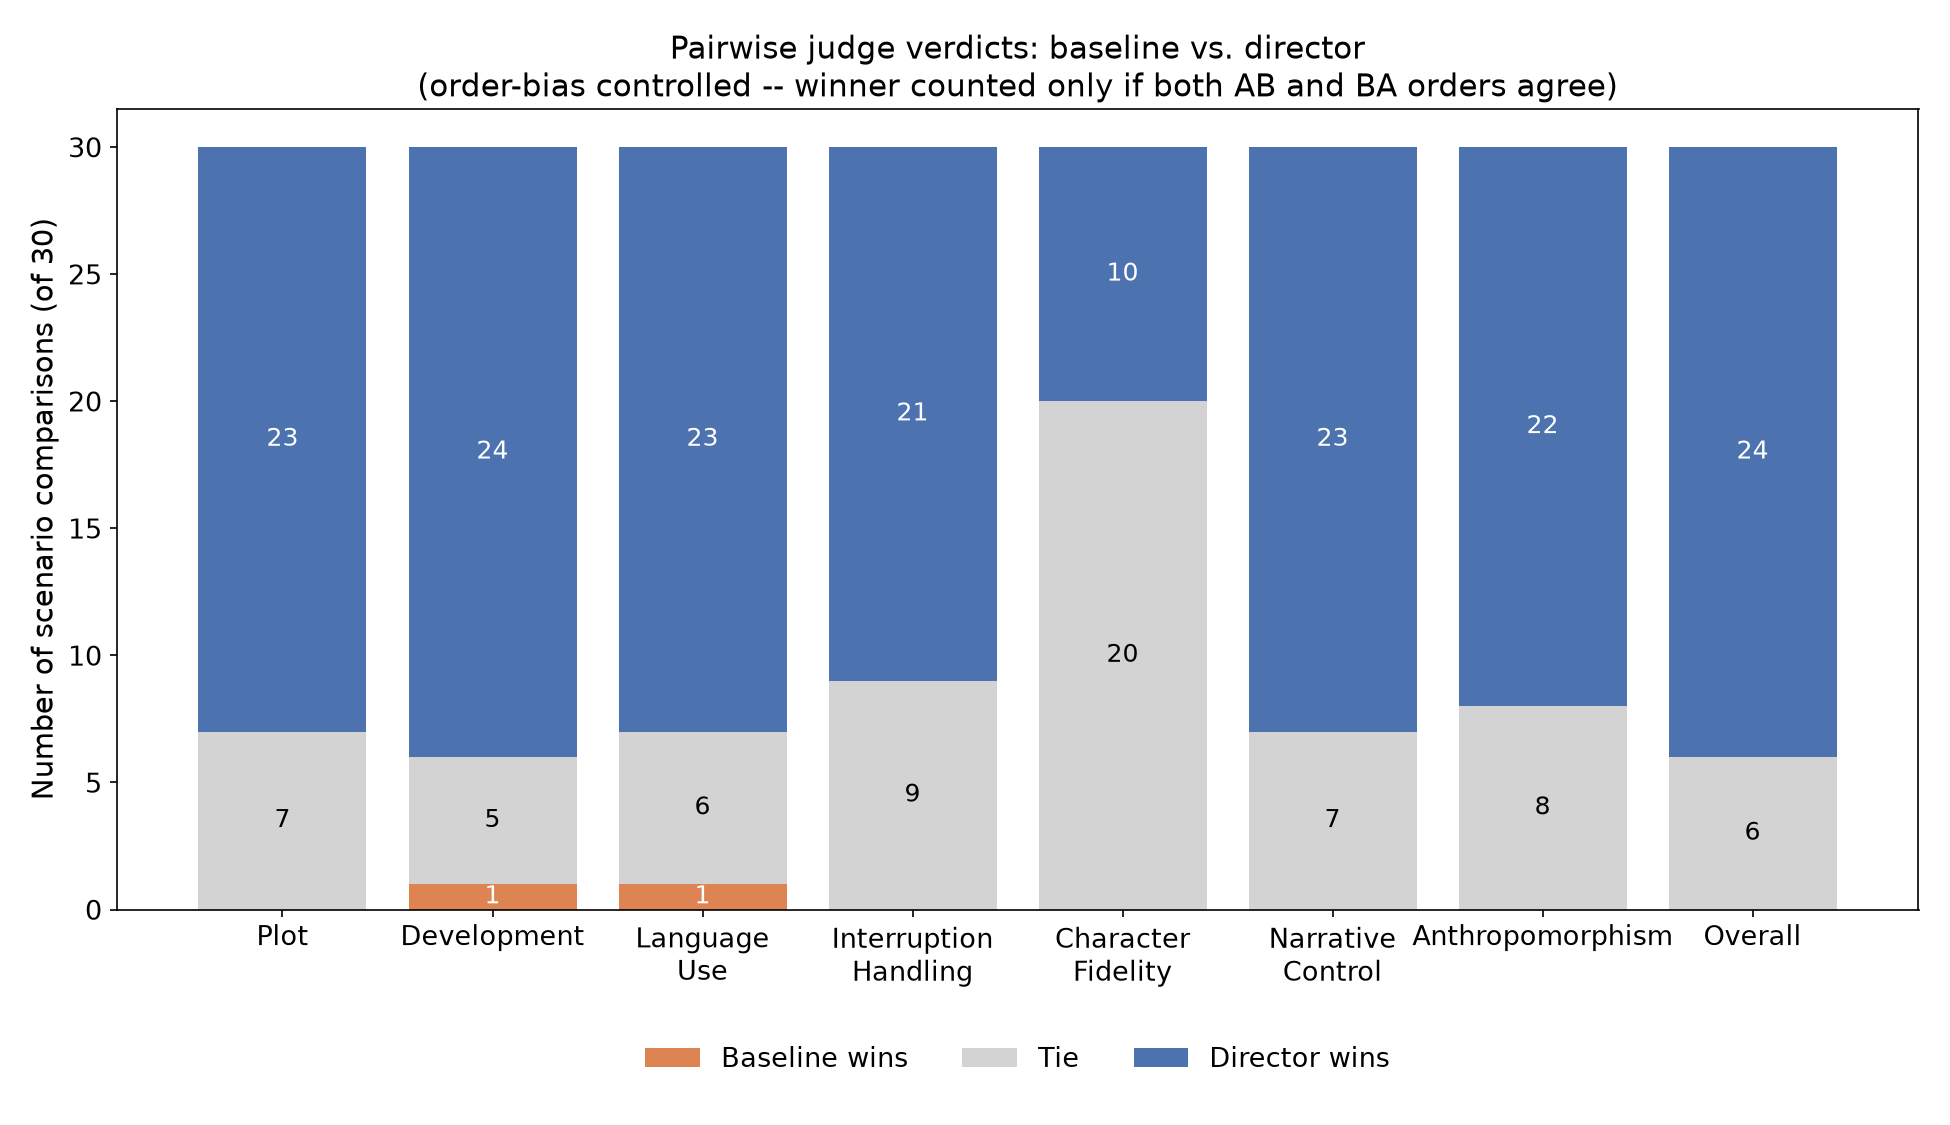
\includegraphics[width=0.95\linewidth]{plots/02_baseline_vs_director_pairwise_wins.png}
\caption{Pairwise verdicts, baseline vs.\ director, order-bias controlled ($n$=30).}
\label{fig:llm-base-wins}
\end{figure}

The pairwise verdicts (Figure~\ref{fig:llm-base-wins}) tell a stricter version of the same story. Because a win only counts when both presentation orders agree, ties dominate every dimension. Where a winner does emerge, it is almost always director.

\begin{quote}
\small
``Story A struggles with handling interruptions, often getting stuck in the same beat and failing to progress the story effectively. Story B handles interruptions more gracefully by acknowledging them and then redirecting back to the story. This approach keeps the narrative on track and maintains coherence.''
\end{quote}

\begin{figure}[htbp]
\centering
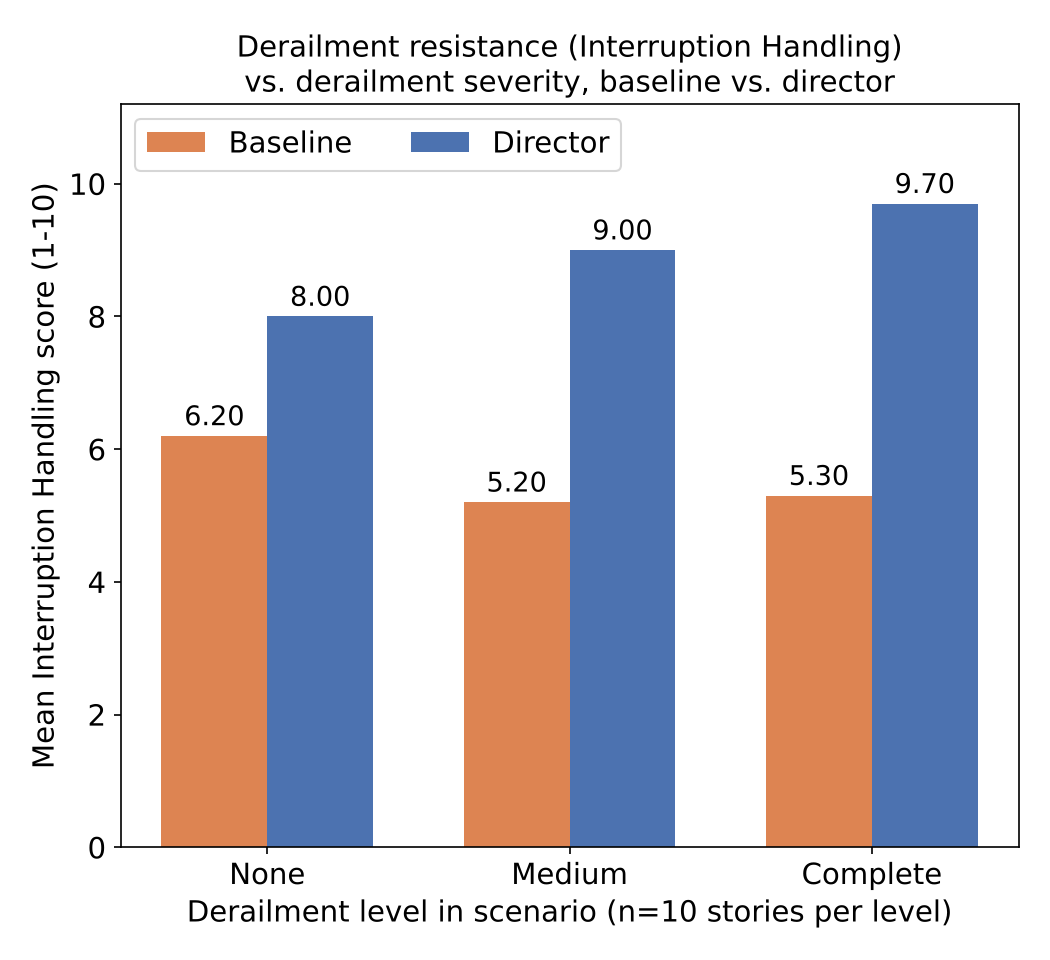
\includegraphics[width=0.6\linewidth]{plots/03_baseline_vs_director_interruption_by_derailment_level.png}
\caption{Interruption Handling score vs.\ derailment severity, baseline vs.\ director, averaged over the Olaf stories at each derailment level.}
\label{fig:llm-base-derail}
\end{figure}

Figure~\ref{fig:llm-base-derail} shows how well each system handles interruptions as the derailment gets more severe. The baseline performs worse the more often the user derails: its Interruption Handling score falls from 6.18 with no derailment to 5.27 at medium and 5.18 at complete derailment. The director does not degrade: its score rises from 8.09 to 8.82 and 9.27, so its lead over the baseline grows from 1.91 to 3.55 and 4.09 points. With no derailment there is little to handle, while repeated derailment is exactly the situation the director is built for and the one in which the baseline struggles most. Averaged over all three derailment levels, the Overall score shows the same picture (5.4 vs.\ 8.5, Figure~\ref{fig:llm-base-metric}).

\textbf{Adversarial and targeted derailment.} For Frozen and Cinderella, we also compared the two systems under the two harder derailment categories described in Section~\ref{sec:characters}. Table~\ref{tab:llm-olaf-advtgt} shows the result. The Director scores higher than the baseline in every scenario, and in the pairwise verdicts the baseline does not win a single dimension. Targeted derailment, where every input tries to end the story, hurts the baseline most (Overall 4.4 to 5.2), while the Director stays between 8.4 and 8.8.

\begin{table}[htbp]
\centering
\caption{Baseline vs.\ director for Olaf under adversarial and targeted derailment: single-story Overall score (0--10) and the number of the eight dimensions won by the director (D) and the baseline (B), or tied, in the order-bias-controlled pairwise comparison. The Overall scores are averaged over five runs; the pairwise columns are counts of dimensions won.}
\label{tab:llm-olaf-advtgt}
\begin{tabular}{llccc}
\toprule
Story & Variant & Baseline & Director & Pairwise wins \\
 & & & & (D / B / tie) \\
\midrule
Frozen     & medium adversarial   & 6.2 & 8.8 & 8 / 0 / 0 \\
Frozen     & complete adversarial & 6.4 & 8.7 & 8 / 0 / 0 \\
Frozen     & medium targeted      & 5.2 & 8.8 & 7 / 0 / 1 \\
Frozen     & complete targeted    & 4.4 & 8.6 & 7 / 0 / 1 \\
\midrule
Cinderella & medium adversarial   & 5.9 & 8.8 & 8 / 0 / 0 \\
Cinderella & complete adversarial & 5.4 & 8.5 & 6 / 0 / 2 \\
Cinderella & medium targeted      & 5.2 & 8.7 & 8 / 0 / 0 \\
Cinderella & complete targeted    & 4.5 & 8.4 & 7 / 0 / 1 \\
\bottomrule
\end{tabular}

\end{table}

\subsection{Director vs.\ CoDi}
\label{sec:llm-codi}

We also compare our Director with CoDi \cite{kim2025codi}, the closest existing director-based system, on the same 30 Olaf transcripts (10 stories at three derailment levels). Besides the core rubric, the judge scores the three dimensions added for this comparison (Table~\ref{tab:rubric}).

\begin{figure}[htbp]
\centering
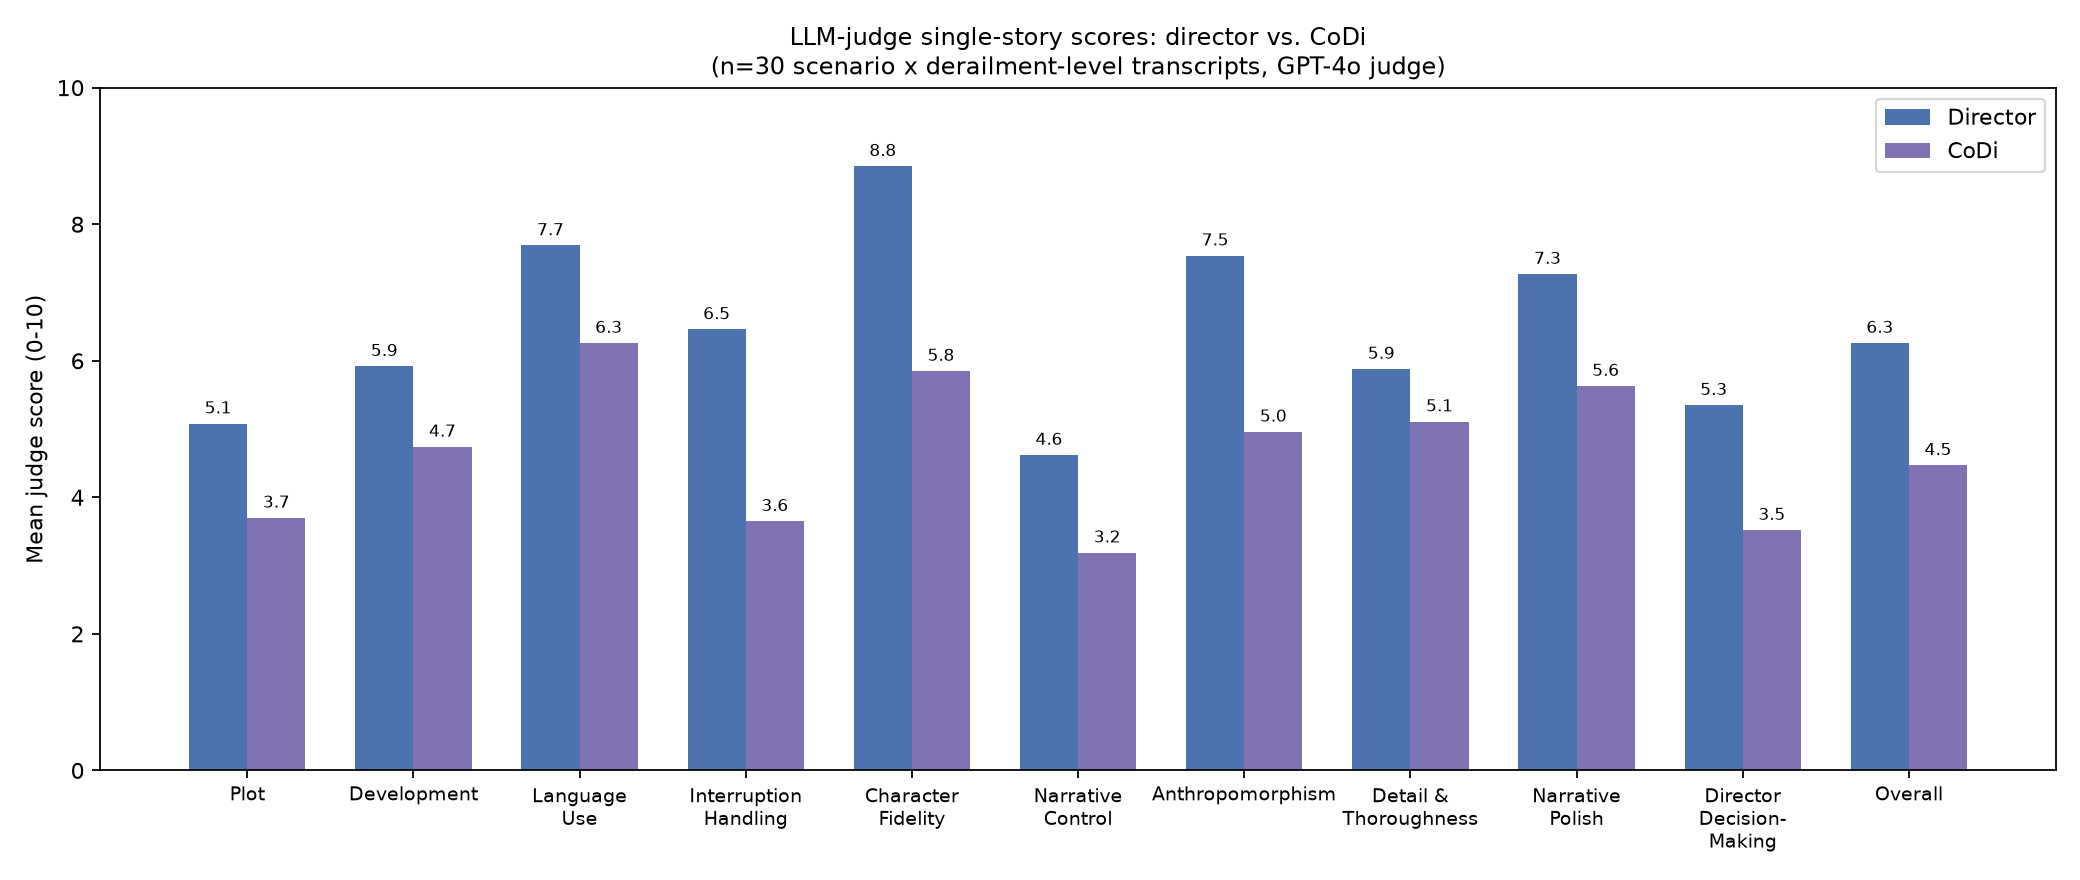
\includegraphics[width=0.95\linewidth]{plots/04_director_vs_codi_scores_by_metric.png}
\caption{Single-story judge scores, director vs.\ CoDi, averaged over all 30 transcripts.}
\label{fig:llm-codi-metric}
\end{figure}

In single-story mode (Figure~\ref{fig:llm-codi-metric}), the Director scores higher than CoDi on every dimension, with an Overall score of 6.3 against 4.5. The largest gaps are on Character Fidelity (8.8 vs.\ 5.8) and Interruption Handling (6.5 vs.\ 3.6), and the smallest on Detail \& Thoroughness (5.9 vs.\ 5.1).

\begin{figure}[htbp]
\centering
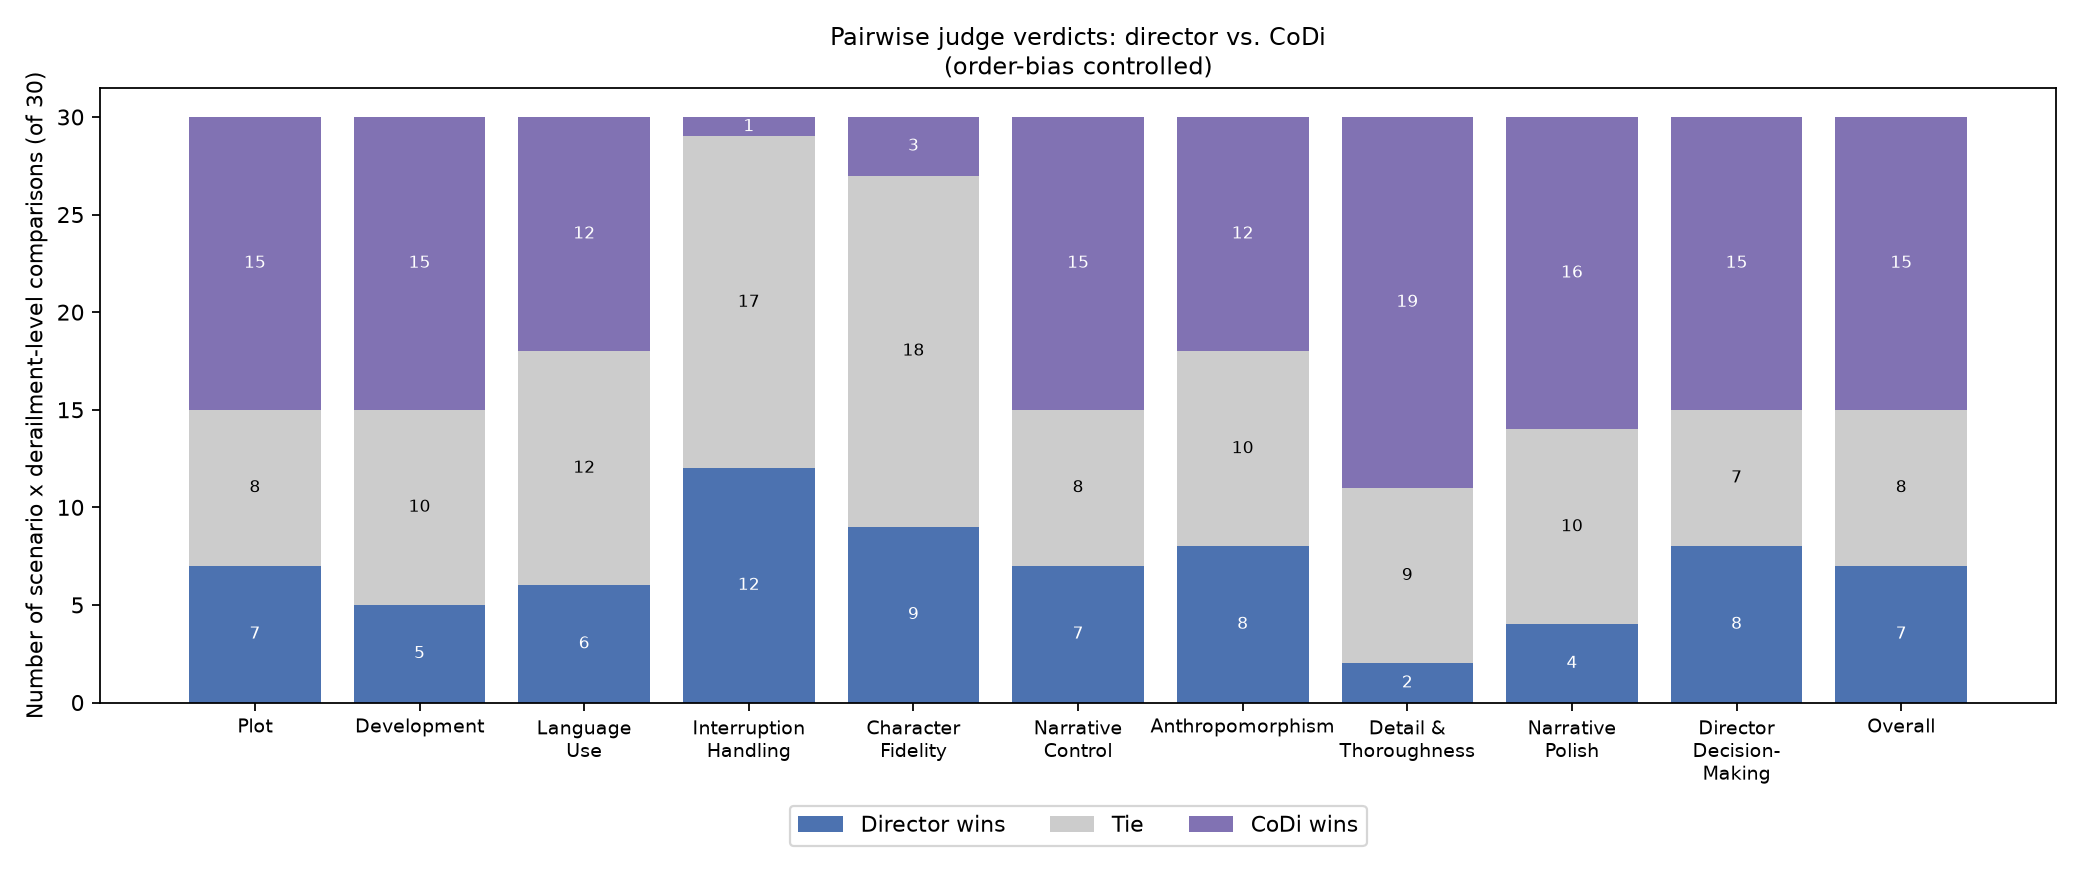
\includegraphics[width=0.95\linewidth]{plots/05_director_vs_codi_pairwise_wins.png}
\caption{Pairwise verdicts, director vs.\ CoDi, order-bias controlled ($n$=30).}
\label{fig:llm-codi-wins}
\end{figure}

The pairwise verdicts (Figure~\ref{fig:llm-codi-wins}) point the other way on most dimensions. CoDi wins more often on Overall (15 vs.\ 7, with 8 ties) and on nine of the eleven dimensions, most clearly on Detail \& Thoroughness (19 vs.\ 2) and Narrative Polish (16 vs.\ 4). The Director wins clearly on Interruption Handling (12 vs.\ 1) and Character Fidelity (9 vs.\ 3), the two dimensions most directly tied to reacting to the user in character.

The two modes disagree because the systems have different goals. CoDi writes complete stories without a live user (Section~\ref{sec:rw-llm-story}), while the Director reacts to a user in real time. We did not run this comparison to show that one system is better, only to show the strengths of each.

Seen this way, the results are consistent. When the judge reads one transcript at a time, it scores each against the rubric, and the Director's handling of interruptions and its stable character voice earn it the higher score. When the judge compares the two transcripts directly, the richer and more finished prose of CoDi stands out and decides the Overall verdict. We therefore read this comparison as showing that the Director handles interruptions and stays in character better than CoDi, while CoDi produces more polished stories when no user interferes.

\section{Ablation Studies}\label{sec:ablation-results}

This section compares the LLM judge with the user study and then varies one part of the setup at a time.

\subsection{User Study vs LLM-as-Judge}
\label{sec:llm-vs-study}

The comparisons above use scenarios the live study never saw, which is the purpose of an automated judge. We can, however, also give the judge the two stories that the participants of the user study played, and check whether the LLM judge and the 14 participants notice the same effects.

The setup of this cross-check and the mapping between the questionnaire and the judge rubric are described in Section~\ref{sec:design-crosscheck}.

\subsubsection{Frozen}

Baseline versus Director on the Frozen story of Section~\ref{sec:story1}.

\begin{table}[htbp]
\centering
\caption{Frozen (\texttt{olaf\_retells\_frozen\_1\_complete\_derailment}), the exact story served in the live study under sustained derailment: judge score, baseline vs.\ director, mean of 5 runs per condition.}
\label{tab:llm-frozen-case}
\begin{tabular}{lcc}
\toprule
Dimension & Baseline & Director \\
\midrule
Plot                    & 3.44 & 8.74 \\
Development             & 4.15 & 8.54 \\
Language Use            & 8.82 & 8.62 \\
Interruption Handling   & 3.88 & 8.89 \\
Character Fidelity      & 8.42 & 8.51 \\
Narrative Control       & 3.12 & 8.54 \\
Anthropomorphism        & 6.55 & 8.86 \\
Overall                 & 5.48 & 8.67 \\
\bottomrule
\end{tabular}
\end{table}

\begin{figure}[htbp]
\centering
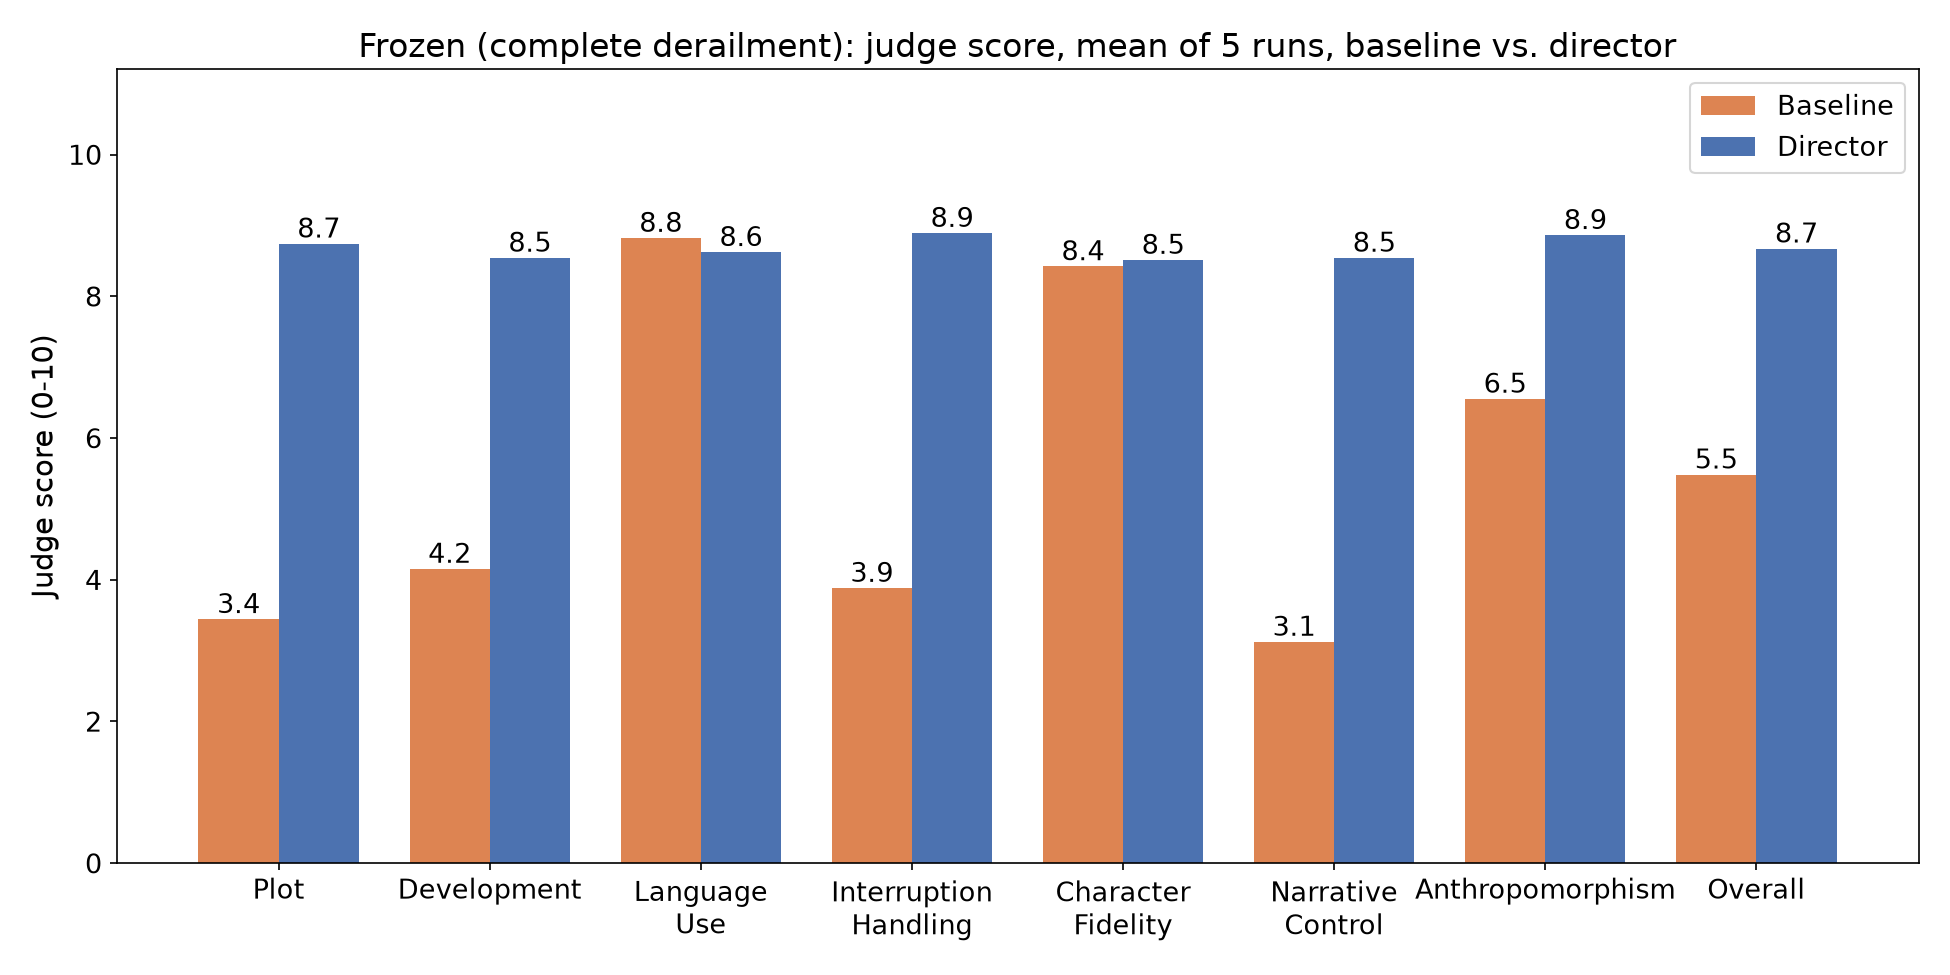
\includegraphics[width=0.95\linewidth]{plots/14_frozen_case_study_complete_derailment.png}
\caption{Frozen, complete derailment: judge score, baseline vs.\ director, mean of 5 runs per condition.}
\label{fig:llm-frozen-case}
\end{figure}

Table~\ref{tab:frozen-side} puts the participants' ratings and the judge scores for each condition next to each other, using the mapping in Table~\ref{tab:question-mapping}. The participants rated on a scale of 1 to 5 and the judge on a scale of 0 to 10, so we compare the direction and relative size of the gaps rather than the raw values.

\begin{table}[htbp]
\centering
\caption{Frozen: user study ratings (1--5, Table~\ref{tab:story1}) and judge scores (0--10, Table~\ref{tab:llm-frozen-case}) for each condition, matched by the mapping in Table~\ref{tab:question-mapping}.}
\label{tab:frozen-side}
\small
\begin{tabular}{llcccc}
\toprule
 & & \multicolumn{2}{c}{User study} & \multicolumn{2}{c}{LLM judge} \\
\cmidrule(lr){3-4} \cmidrule(lr){5-6}
Question & Judge dimension & Baseline & Director & Baseline & Director \\
\midrule
Q1 Coherence    & Plot                  & 1.71 & 3.93 & 3.44 & 8.74 \\
Q2 Character    & Character Fidelity    & 4.00 & 4.29 & 8.42 & 8.51 \\
Q4 Overall      & Overall               & 2.93 & 3.57 & 5.48 & 8.67 \\
Q5a Derailment  & Interruption Handling & 1.58 & 4.42 & 3.88 & 8.89 \\
                & Narrative Control     & 1.58 & 4.42 & 3.12 & 8.54 \\
\bottomrule
\end{tabular}
\end{table}

The two evaluations agree on three of the four questions. Both rate the baseline low and the Director high on coherence and on resisting derailment. For coherence, participants gave the baseline 1.71 and the Director 3.93, and the judge gave 3.44 and 8.74 on Plot. For derailment, participants gave 1.58 and 4.42, and the judge's largest gaps are on the two matching dimensions, Narrative Control (+5.42) and Interruption Handling (+5.01). Both also see almost no difference in staying in character. Participants rated the baseline 4.00 and the Director 4.29, and the judge gave 8.42 and 8.51 on Character Fidelity. The baseline keeps Olaf's voice in both evaluations and loses the plot.

The two evaluations disagree on the overall rating. Participants rated the Director only slightly higher (3.57 vs.\ 2.93, \pval{0.12}), while the judge places the two far apart (8.67 vs.\ 5.48). One reason may be that participants also weigh how the conversation felt, and some found the Director's steering rigid (Section~\ref{sec:story1}). The judge reads a scripted transcript and scores mainly whether the story was told. Language Use is the only judge dimension where the baseline scores slightly higher ($-0.20$). It has no direct counterpart in the questionnaire.

\subsubsection{Cinderella}

Director versus the 5-minute time-constrained Director on the Cinderella story of Section~\ref{sec:story2}. As for Frozen, we use the complete-derailment variant, because participants were asked to derail the story constantly. We also ran the baseline on this story, which the user study did not include for Cinderella.

\begin{table}[htbp]
\centering
\caption{Cinderella (\texttt{olaf\_retells\_cinderella\_complete\_derailment}), the exact story served in the live study under sustained derailment: judge score, mean of 5 runs per condition. 5 min is the same budget as in the live study's time-constrained condition.}
\label{tab:llm-cinderella-case}
\begin{tabular}{lccc}
\toprule
Dimension & Baseline & Director & 5 min \\
\midrule
Plot                    & 4.8 & 9.0  & 8.8 \\
Development             & 5.8 & 8.4  & 8.6 \\
Language Use            & 7.6 & 9.2  & 9.4 \\
Interruption Handling   & 5.6 & 9.8  & 9.4 \\
Character Fidelity      & 8.6 & 10.0 & 10.0 \\
Narrative Control       & 4.4 & 9.0  & 8.8 \\
Anthropomorphism        & 7.4 & 9.2  & 9.6 \\
\midrule
Overall                 & 6.2 & 9.1  & 9.1 \\
\bottomrule
\end{tabular}
\end{table}

\begin{figure}[htbp]
\centering
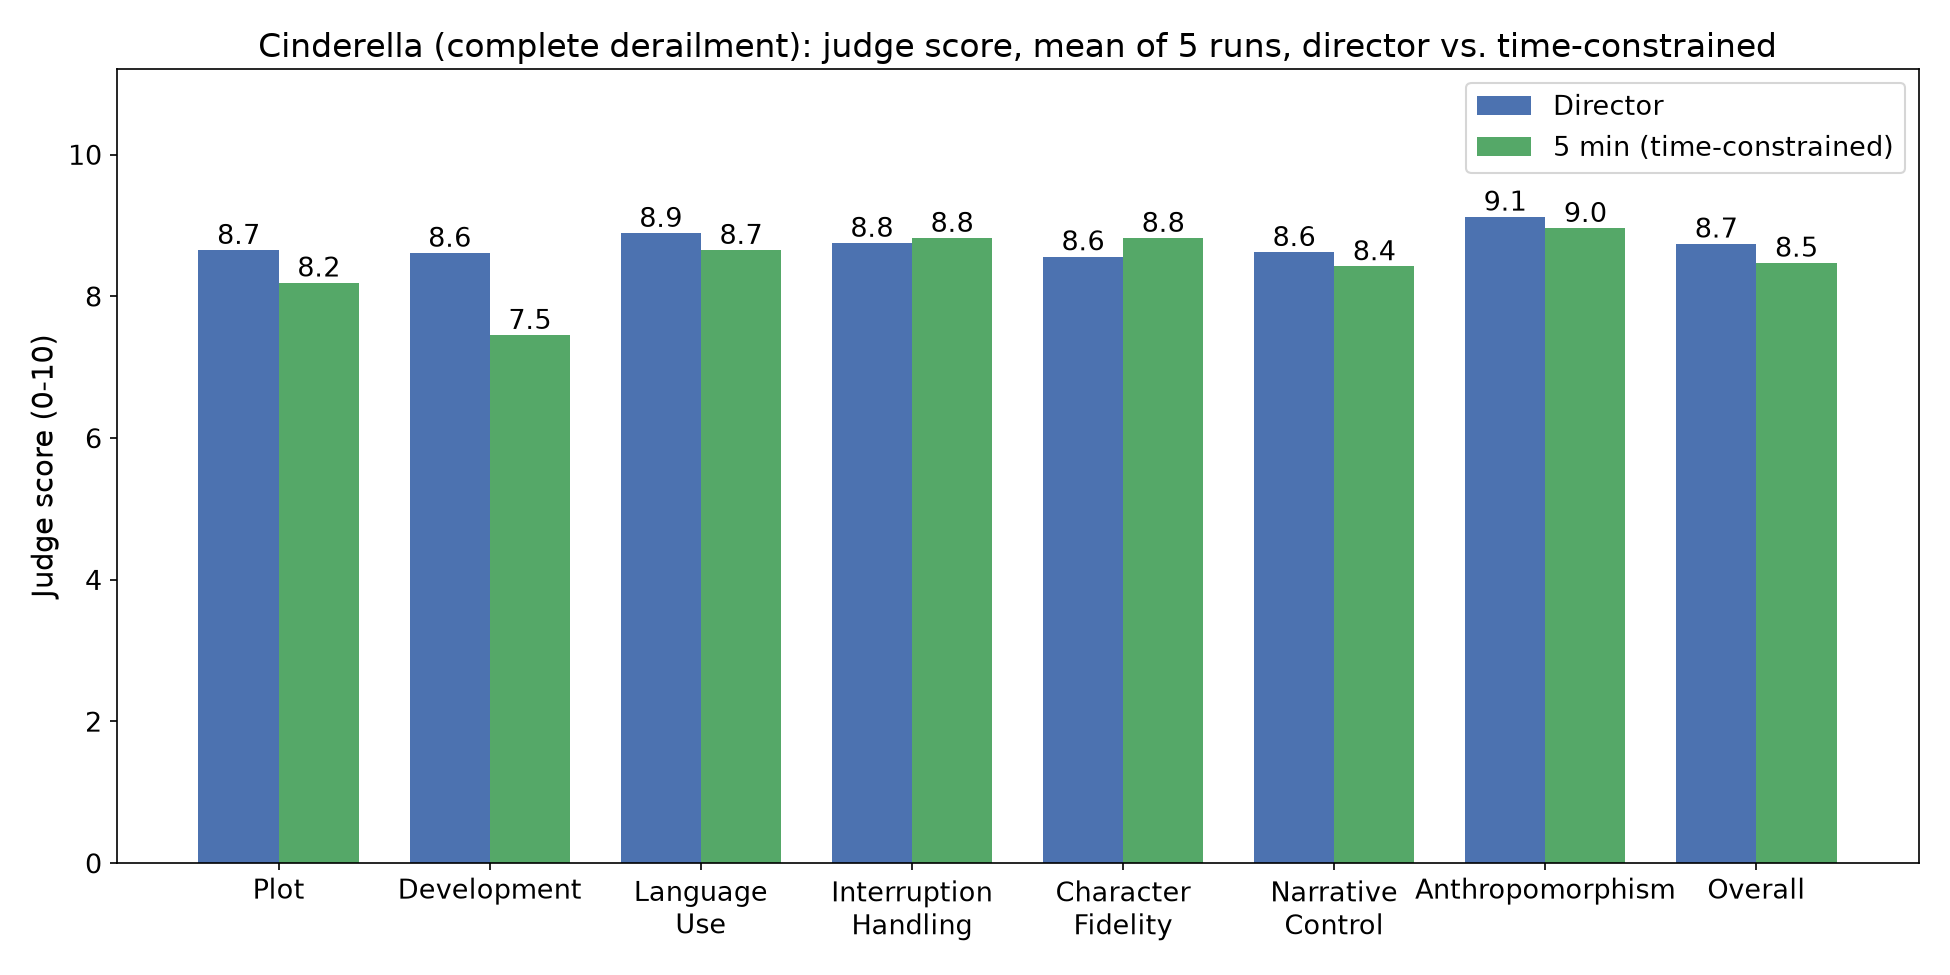
\includegraphics[width=0.95\linewidth]{plots/15_cinderella_case_study_complete_derailment.png}
\caption{Cinderella, complete derailment: judge score, baseline, director and the 5-minute time-constrained director, mean of 5 runs per condition.}
\label{fig:llm-cinderella-case}
\end{figure}

Table~\ref{tab:cinderella-side} again puts the two evaluations side by side.

\begin{table}[htbp]
\centering
\caption{Cinderella: user study ratings (1--5, Tables~\ref{tab:story2} and~\ref{tab:ending}) and judge scores (0--10, Table~\ref{tab:llm-cinderella-case}) for each condition, matched by the mapping in Table~\ref{tab:question-mapping}. TC is the 5-minute time-constrained Director.}
\label{tab:cinderella-side}
\small
\begin{tabular}{llcccc}
\toprule
 & & \multicolumn{2}{c}{User study} & \multicolumn{2}{c}{LLM judge} \\
\cmidrule(lr){3-4} \cmidrule(lr){5-6}
Question & Judge dimension & Director & TC & Director & TC \\
\midrule
Q1 Coherence    & Plot                  & 3.79 & 3.71 & 9.0 & 8.8 \\
Q2 Character    & Character Fidelity    & 4.14 & 4.14 & 10.0 & 10.0 \\
Q4 Overall      & Overall               & 3.36 & 3.29 & 9.1 & 9.1 \\
Q5a Derailment  & Interruption Handling & 4.07 & 3.75 & 9.8 & 9.4 \\
                & Narrative Control     & 4.07 & 3.75 & 9.0 & 8.8 \\

\bottomrule
\end{tabular}
\end{table}

On the core questions, both evaluations find the two conditions close. Participants rated them within 0.32 points on every question, and none of the differences is significant (all $p \ge 0.40$). The judge places them within 0.4 points on every dimension and gives both the same Overall score (9.1). Both stay fully in character (10.0 on Character Fidelity), and the largest differences are small: the Director is ahead on Interruption Handling (9.8 vs.\ 9.4) and the time-constrained Director on Anthropomorphism (9.6 vs.\ 9.2). The baseline, which only the judge evaluated on this story, falls far behind both (Overall 6.2), with the same weaknesses as on Frozen: low scores on Narrative Control (4.4), Plot (4.8) and Interruption Handling (5.6), but a high score on Character Fidelity (8.6).

\subsection{Character Ablation: Rocket Raccoon}
\label{sec:llm-rocket}

Every comparison so far uses Olaf as the character. A system whose director layer only works for one character's voice would be a weak result, so we repeated the baseline-vs-director comparison from Section~\ref{sec:llm-baseline} on a second character with a deliberately different personality: Rocket Raccoon, whose defensive, sarcastic, deflecting register is close to the opposite of Olaf's earnest, naive one. None of the director's rules (bridge sentences, anti-stall pacing, staying in character under derailment) are written with Olaf specifically in mind, i.e.\ they are character-agnostic, so this is a direct test of whether the director's advantage generalizes to other characters.

We built a Red Riding Hood suite for Rocket with the same seven variants as for Olaf (Section~\ref{sec:characters}), judged with the same rubric and order-bias-controlled protocol (Section~\ref{sec:design-judge}). All results below cover the 7 scenarios, including the adversarial and targeted ones.

\begin{figure}[htbp]
\centering
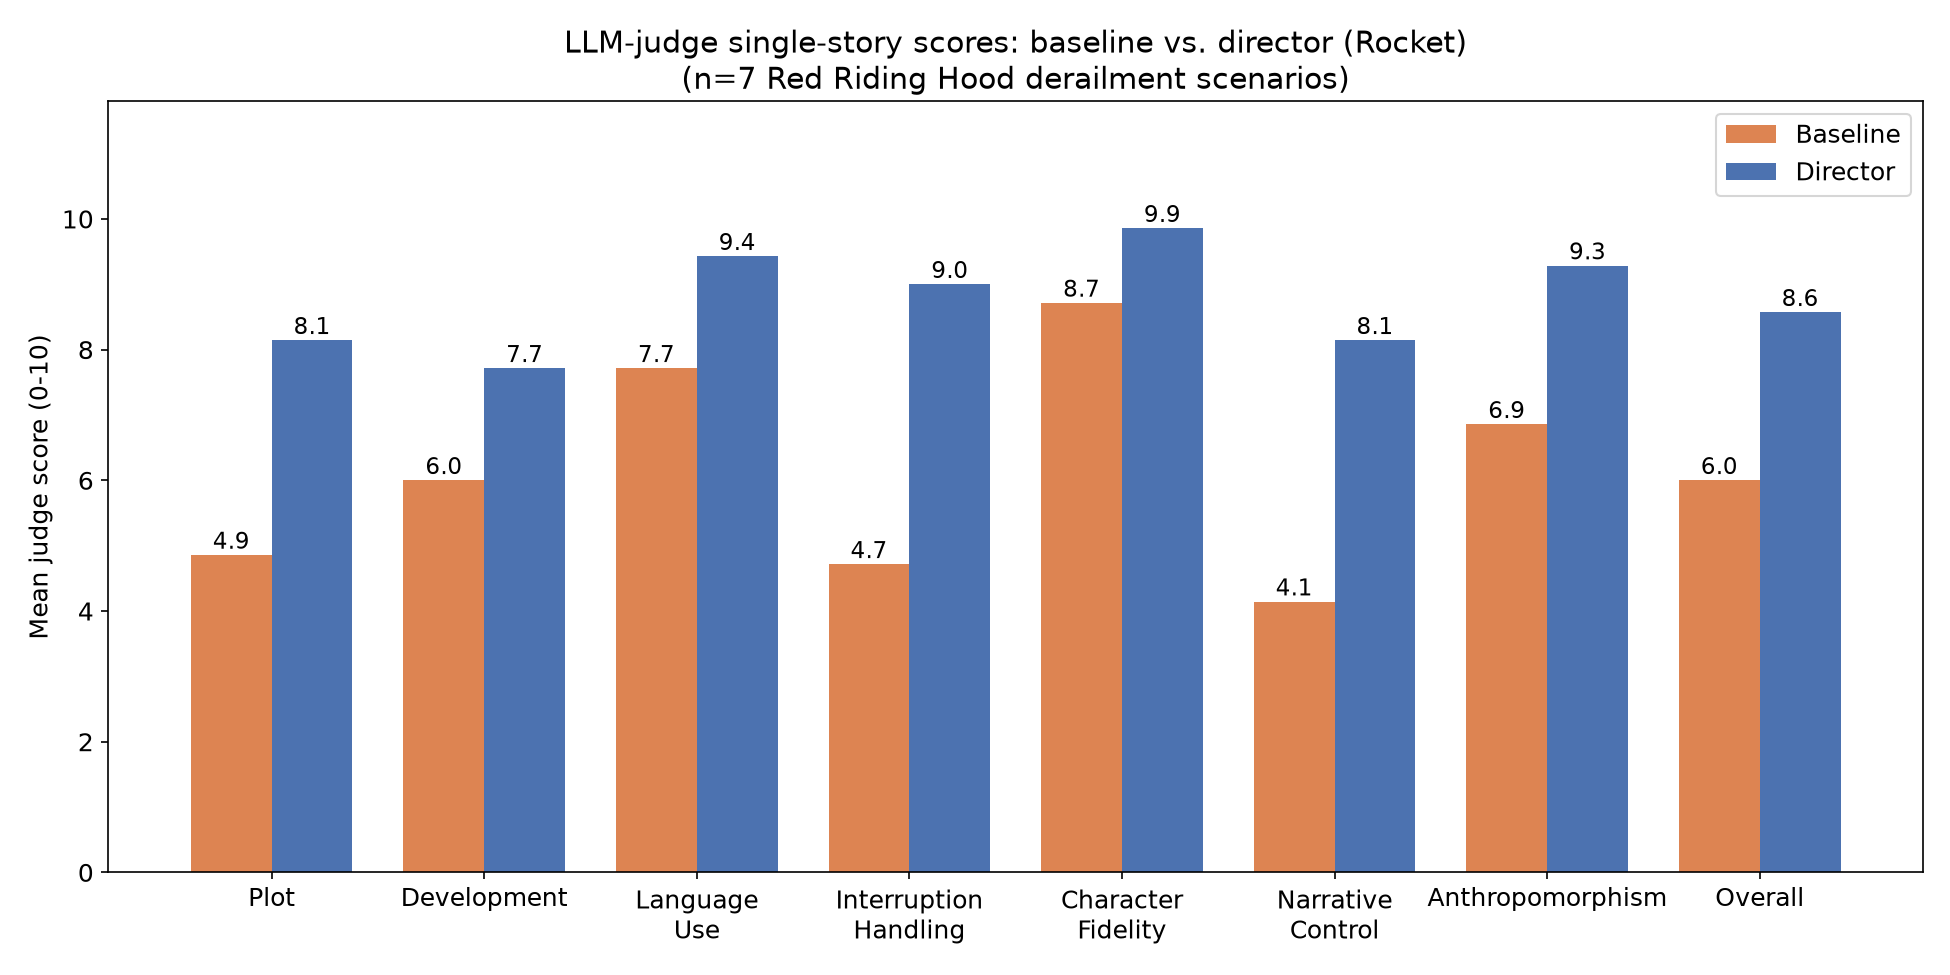
\includegraphics[width=0.95\linewidth]{plots/08_rocket_scores_by_metric.png}
\caption{Single-story judge scores, baseline vs.\ director, Rocket, averaged over all 7 transcript pairs.}
\label{fig:llm-rocket-metric}
\end{figure}

\begin{table}[htbp]
\centering
\caption{Single-story judge scores, baseline vs.\ director for Rocket, averaged over all 7 scenarios.}
\label{tab:llm-rocket-metric}
\begin{tabular}{lcc}
\toprule
Dimension & Baseline & Director \\
\midrule
Plot                  & 4.9 & 8.2 \\
Development           & 6.1 & 7.8 \\
Language Use          & 7.7 & 9.4 \\
Interruption Handling & 4.6 & 8.9 \\
Character Fidelity    & 8.7 & 9.8 \\
Narrative Control     & 4.2 & 8.2 \\
Anthropomorphism      & 6.8 & 9.3 \\
\midrule
Overall               & 6.1 & 8.8 \\
\bottomrule
\end{tabular}
\end{table}

Figure~\ref{fig:llm-rocket-metric} and Table~\ref{tab:llm-rocket-metric} show that the pattern from Olaf holds for Rocket, and more strongly. The director scores higher than the baseline on every dimension, with an Overall score of 8.8 against 6.1. The largest gaps are on Interruption Handling (8.9 vs.\ 4.6) and Narrative Control (8.2 vs.\ 4.2), followed by Plot (8.2 vs.\ 4.9). The smallest gap is on Character Fidelity (9.8 vs.\ 8.7), where the baseline already stays close to Rocket's voice. The pairwise verdicts (Figure~\ref{fig:llm-rocket-wins}) are almost unanimous, with the director winning on nearly every dimension.

\begin{figure}[htbp]
\centering
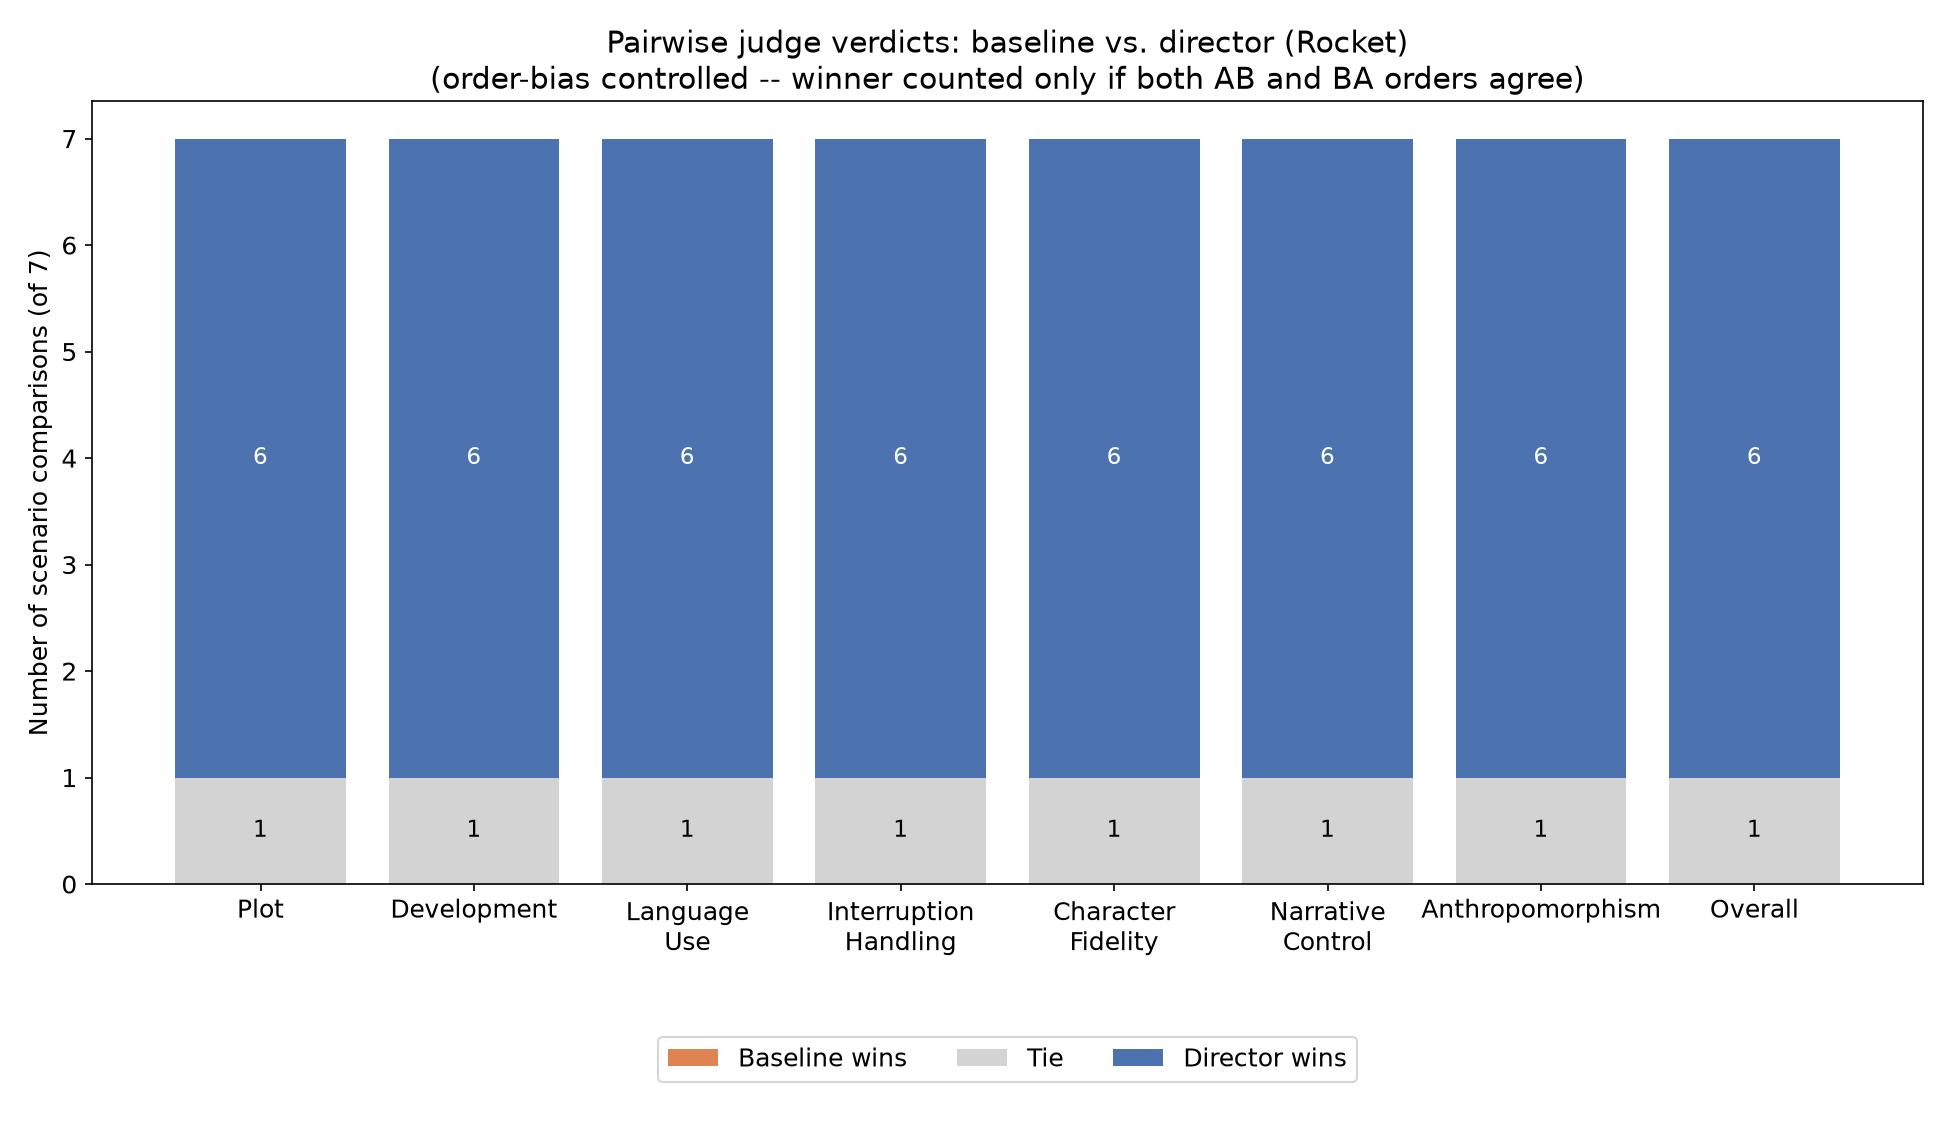
\includegraphics[width=0.95\linewidth]{plots/09_rocket_pairwise_wins.png}
\caption{Pairwise verdicts, baseline vs.\ director, Rocket, order-bias controlled }
\label{fig:llm-rocket-wins}
\end{figure}

Breaking the results down by derailment level (Figure~\ref{fig:llm-rocket-derail} and Table~\ref{tab:llm-rocket-derail}) shows that the director's advantage for Rocket does not shrink under heavier derailment: it stays at 2.5 to 2.7 points from medium through complete derailment, in line with the growing lead in Interruption Handling for Olaf (Figure~\ref{fig:llm-base-derail}). The ``none'' cell here is a single scenario, not an average, and one baseline single-story score at the complete level failed to parse and was excluded from that cell's mean (n=2 instead of 3). This rests on far fewer scenarios per cell than the Olaf results, so it should be read as directional, not conclusive.

\begin{figure}[htbp]
\centering
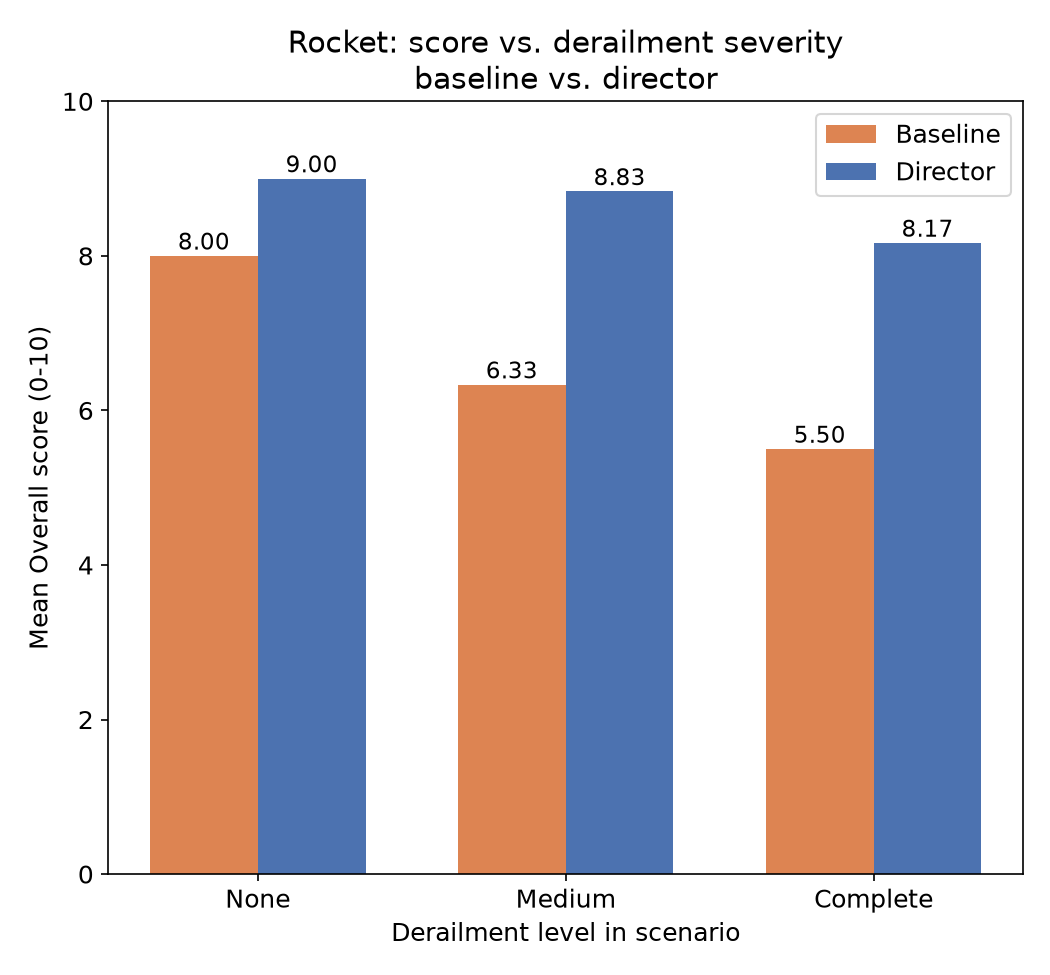
\includegraphics[width=0.65\linewidth]{plots/10_rocket_by_derailment_level.png}
\caption{Overall score vs.\ derailment severity, baseline vs.\ director.}
\label{fig:llm-rocket-derail}
\end{figure}

\begin{table}[htbp]
\centering
\caption{Rocket: Overall score by derailment level.}
\label{tab:llm-rocket-derail}
\begin{tabular}{lccc}
\toprule
 & None & Medium & Complete \\
\midrule
Baseline & 8.00 & 6.33 & 5.50 \\
Director & 9.00 & 8.83 & 8.17 \\
\bottomrule
\end{tabular}
\end{table}

Taken together, this suggests that the director's advantage over baseline is not specific to Olaf's character prompt.

\subsection{Narrative Representation Ablation}
\label{sec:llm-beats-ablation}

This section compares the beat-based Director with the full-text variant described in Section~\ref{sec:ablations}. We ran both directors (beats and full-text) on the same Red Riding Hood derailment scenarios used in Section~\ref{sec:llm-rocket}, with Olaf, and judged the pairs head-to-head with the same AB/BA-controlled protocol as everywhere else in this chapter.

\begin{figure}[htbp]
\centering
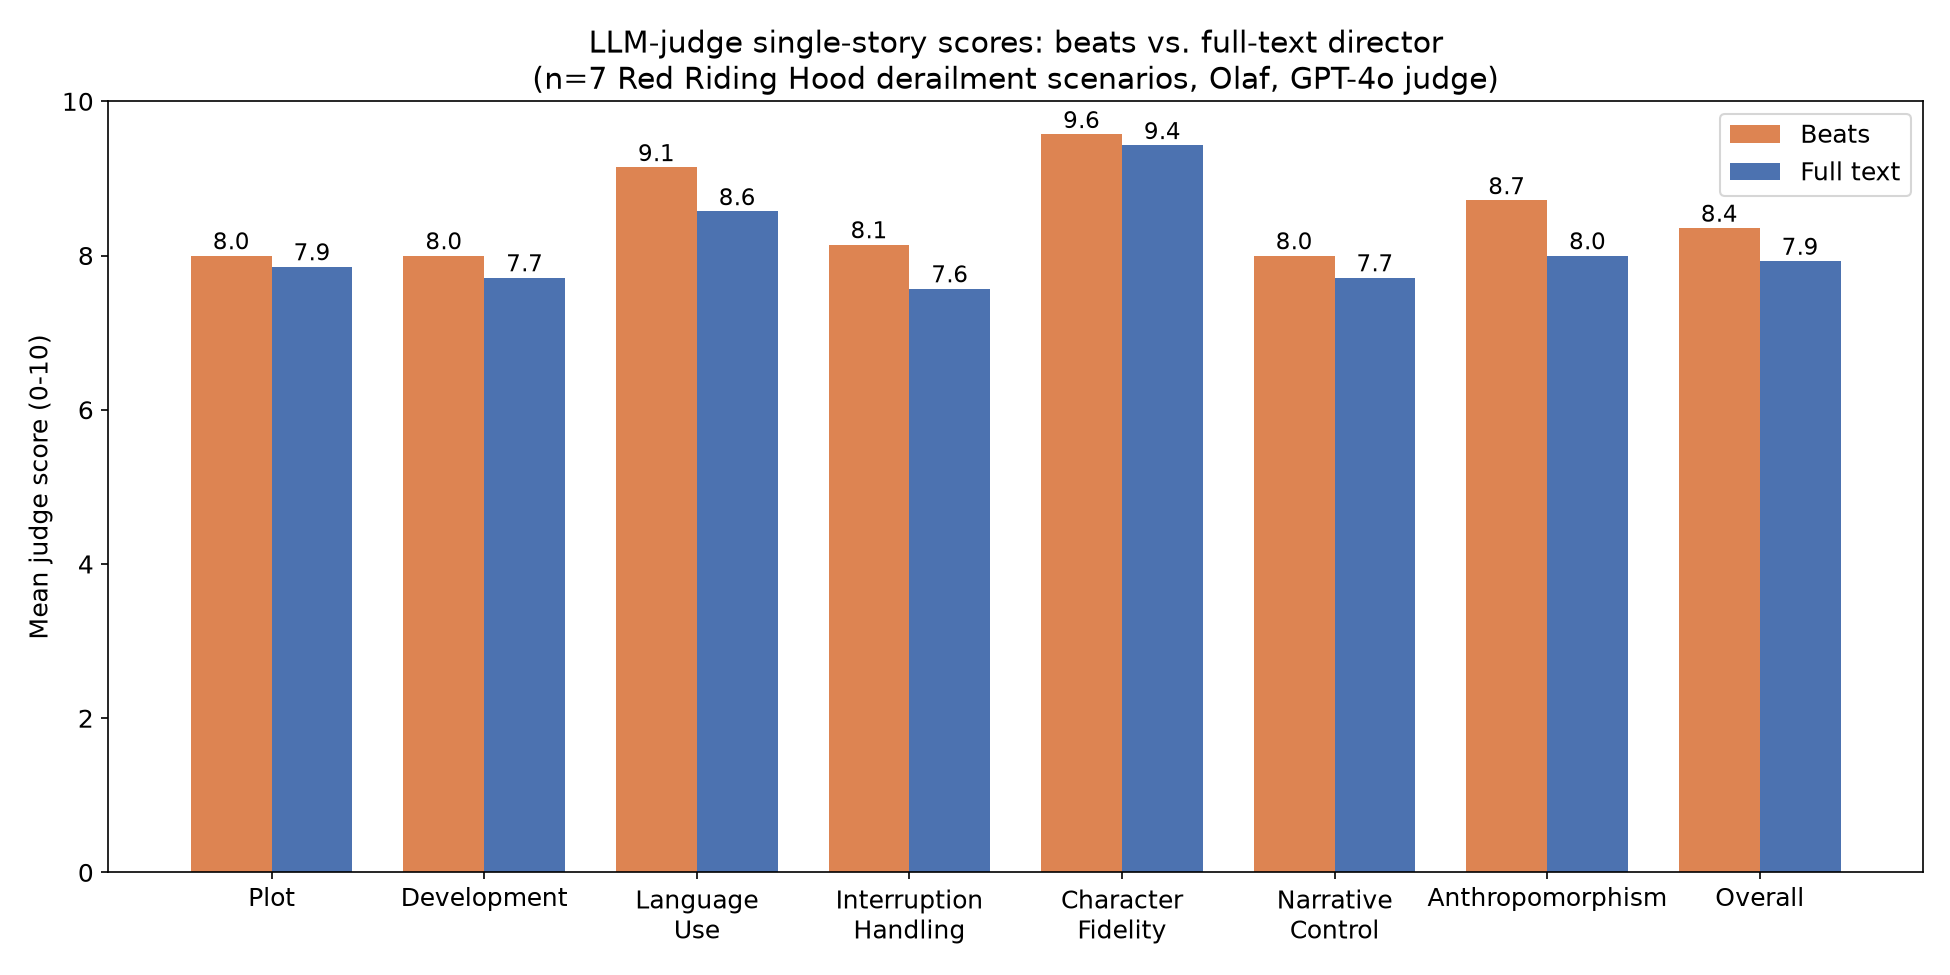
\includegraphics[width=0.95\linewidth]{plots/11_beats_vs_fulltext_scores_by_metric.png}
\caption{Single-story judge scores, beats vs.\ full-text director}
\label{fig:llm-beats-metric}
\end{figure}

\begin{table}[htbp]
\centering
\caption{Beats-based director vs.\ full-text director, mean single-story score per dimension.}
\label{tab:llm-beats-metric}
\begin{tabular}{lcc}
\toprule
Dimension & Beats & Full text \\
\midrule
Plot                   & 8.00 & 7.86 \\
Development             & 8.00 & 7.71 \\
Language Use            & 9.14 & 8.57 \\
Interruption Handling   & 8.14 & 7.57 \\
Character Fidelity      & 9.57 & 9.43 \\
Narrative Control       & 8.00 & 7.71 \\
Anthropomorphism        & 8.71 & 8.00 \\
Overall                  & 8.36 & 7.93 \\
\bottomrule
\end{tabular}
\end{table}

Beats score higher on every dimension (Figure~\ref{fig:llm-beats-metric}, Table~\ref{tab:llm-beats-metric}), though the margins are smaller than against the baseline. The Overall score is 8.36 for beats and 7.93 for full text. The largest gaps are on Anthropomorphism (8.71 vs.\ 8.00), Language Use (9.14 vs.\ 8.57) and Interruption Handling (8.14 vs.\ 7.57), while Plot and Character Fidelity differ by only 0.14 points. Both conditions have a full director layer doing the interruption-handling work, so this ablation isolates the story-representation choice specifically. The pairwise verdicts (Figure~\ref{fig:llm-beats-wins}) make the direction unambiguous even though the margins are modest: beats wins or ties every pairwise verdict. Per-scenario Overall (Figure~\ref{fig:llm-beats-scenario}, Table~\ref{tab:llm-beats-scenario}) shows the same pattern: in the pairwise verdicts, beats wins outright on 2 of 7 scenarios and ties the other 5. On single-story scores, full text scores higher on only one scenario (\texttt{complete\_adversarial}, 9.0 vs.\ 8.0).

\begin{figure}[htbp]
\centering
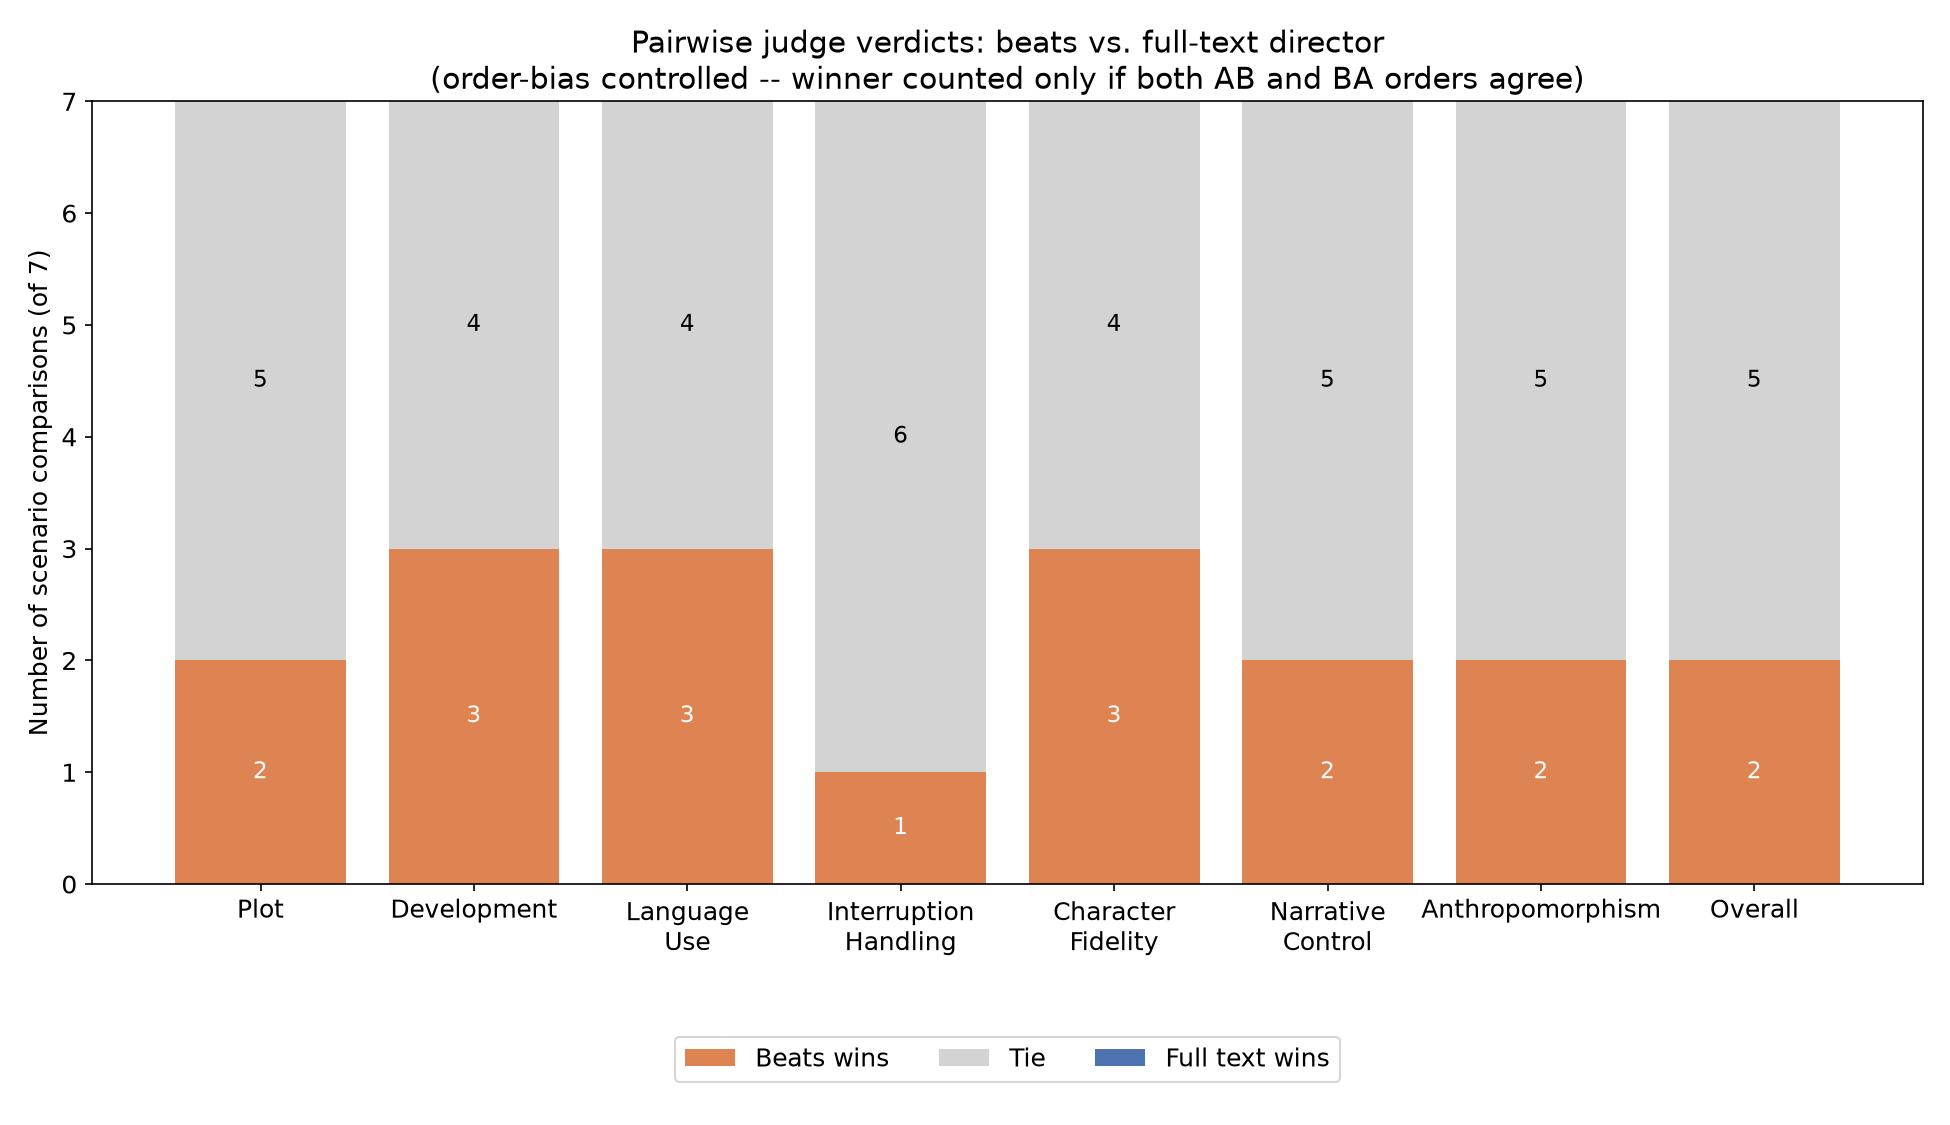
\includegraphics[width=0.95\linewidth]{plots/12_beats_vs_fulltext_pairwise_wins.png}
\caption{Pairwise verdicts, beats vs.\ full-text director, order-bias controlled.}
\label{fig:llm-beats-wins}
\end{figure}

\begin{figure}[htbp]
\centering
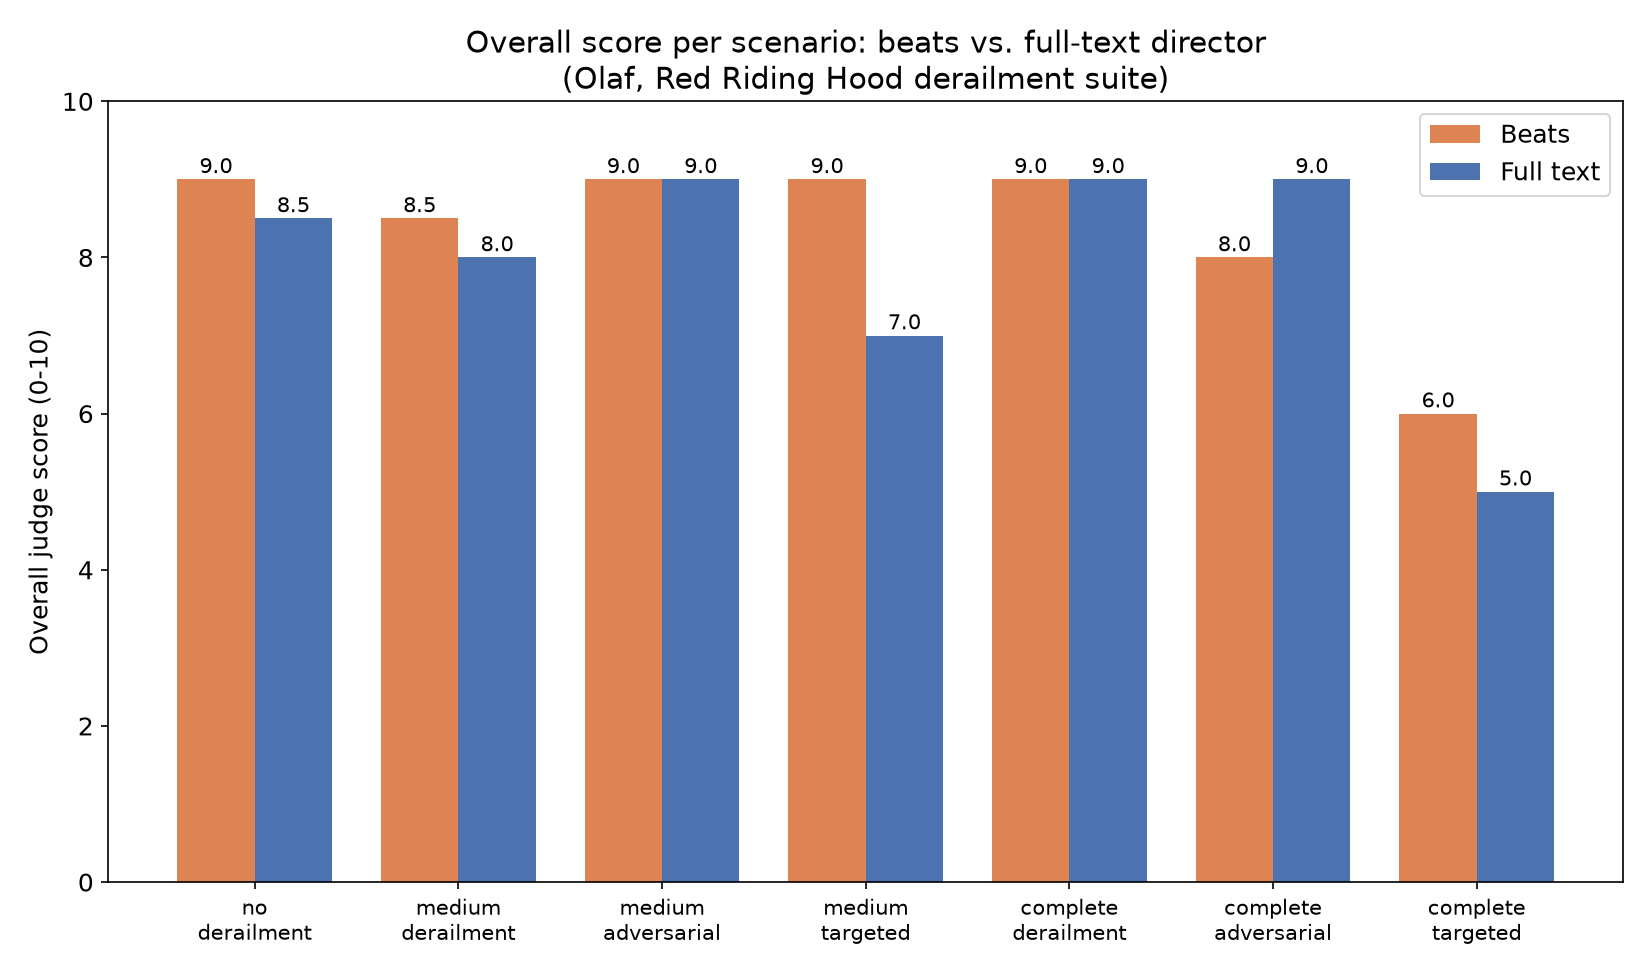
\includegraphics[width=0.95\linewidth]{plots/13_beats_vs_fulltext_by_scenario.png}
\caption{Overall score per scenario, beats vs.\ full-text director.}
\label{fig:llm-beats-scenario}
\end{figure}

\begin{table}[htbp]
\centering
\caption{Overall score per scenario, beats vs.\ full-text director.}
\label{tab:llm-beats-scenario}
\begin{tabular}{lccc}
\toprule
Scenario & Beats & Full text & AB/BA winner \\
\midrule
no\_derailment              & 9.0 & 8.5 & Tie \\
medium\_derailment          & 8.5 & 8.0 & Tie \\
medium\_adversarial         & 9.0 & 9.0 & Tie \\
medium\_targeted            & 9.0 & 7.0 & Beats \\
complete\_derailment        & 9.0 & 9.0 & Beats \\
complete\_adversarial       & 8.0 & 9.0 & Tie \\
complete\_targeted          & 6.0 & 5.0 & Tie \\
\bottomrule
\end{tabular}
\end{table}

\subsection{Time-Budget Ablation}
\label{sec:llm-timebudget}

To see how the time budget affects the story, we ran the Time-Constrained Director with limits of 0.5, 2, 5 and 10 minutes at all three derailment levels. Table~\ref{tab:llm-timebudget} and Figure~\ref{fig:llm-timebudget} show the Overall judge score.

\begin{table}[htbp]
\centering
\caption{Time-budget ablation: Overall judge score (0--10) by time limit and derailment level, with the approximate number of turns the story lasts.}
\label{tab:llm-timebudget}
\begin{tabular}{lcccc}
\toprule
Time limit & Approx.\ turns & No derailment & Medium & Complete \\
\midrule
0.5 min       & 1--2   & 4.60 & 4.40 & 4.10 \\
2 min         & 5--6   & 7.30 & 6.90 & 6.50 \\
5 min         & 12--14 & 8.80 & 8.70 & 8.50 \\
10 min        & 20     & 8.70 & 8.60 & 8.60 \\
\bottomrule
\end{tabular}
\end{table}

\begin{figure}[htbp]
\centering
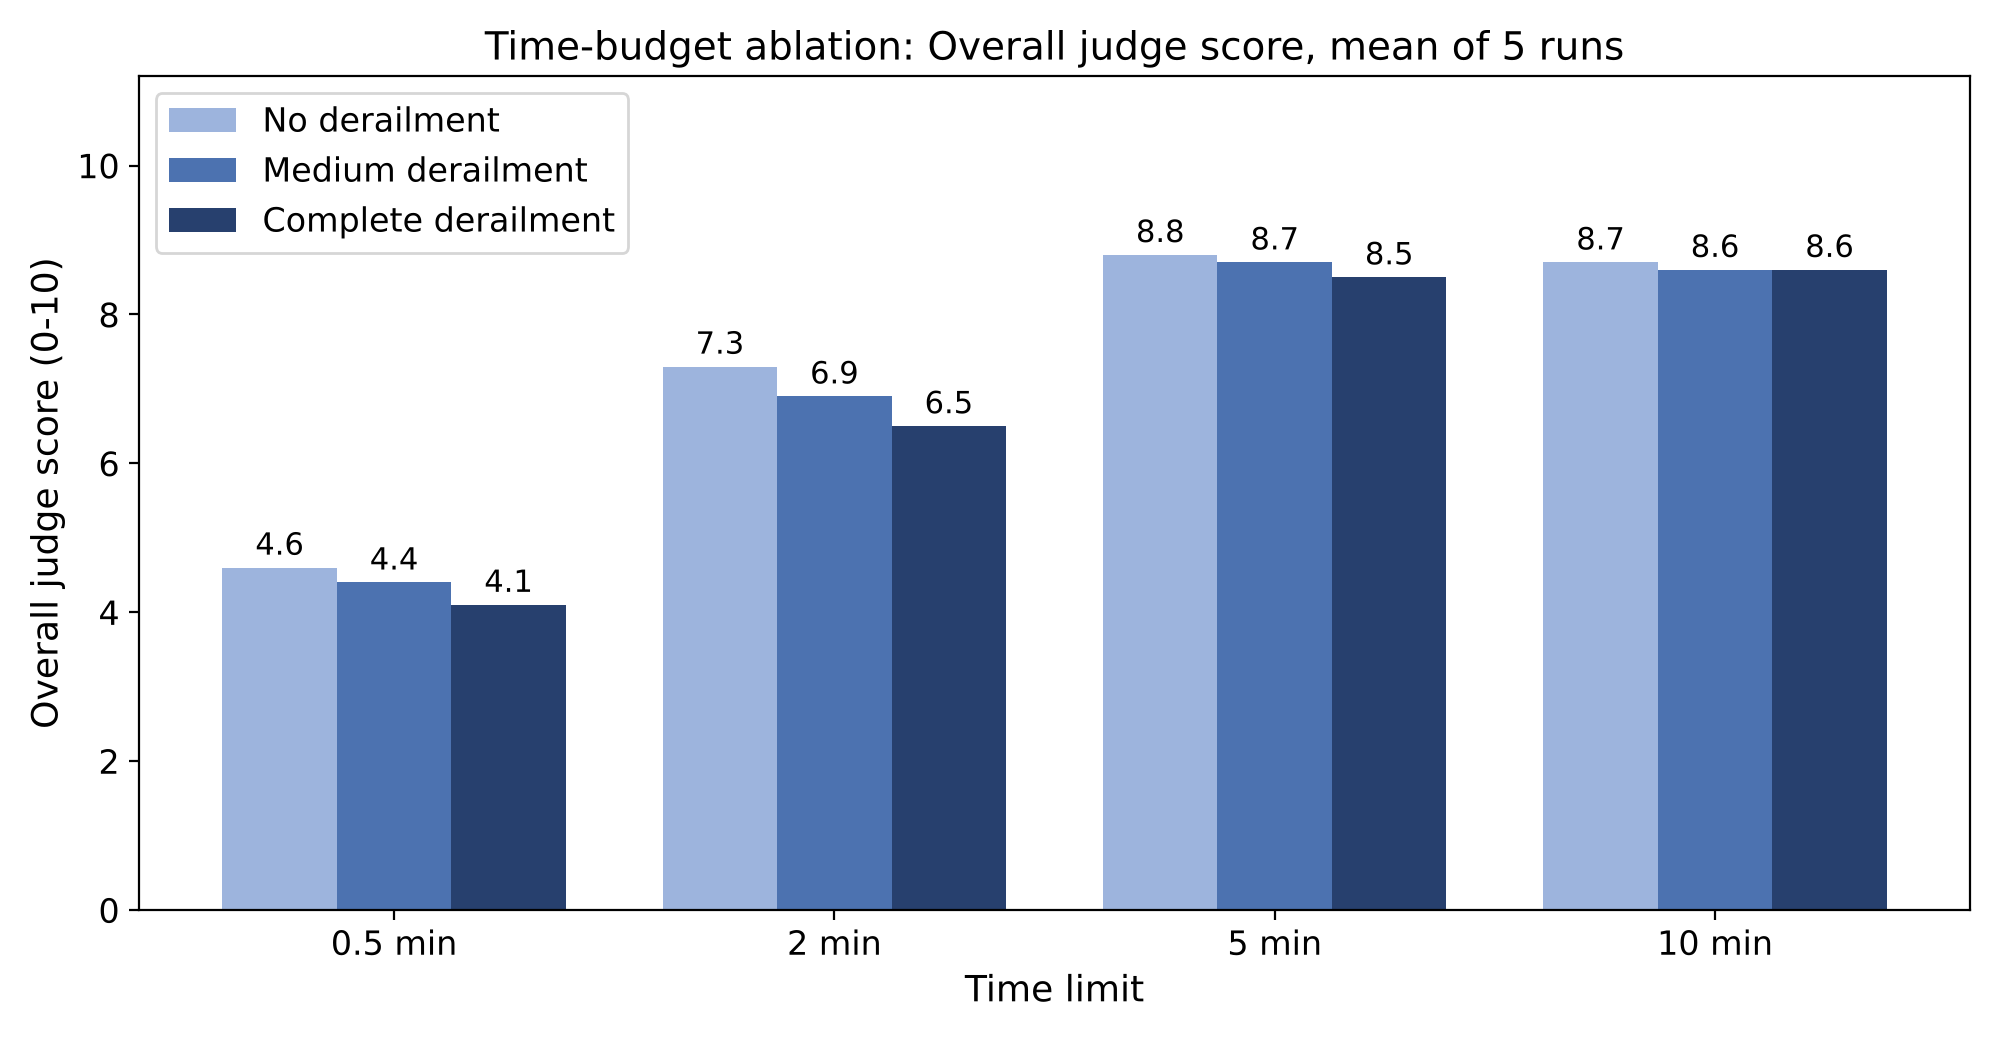
\includegraphics[width=0.95\linewidth]{plots/18_time_budget_ablation.png}
\caption{Time-budget ablation: Overall judge score by time limit, for the three derailment levels.}
\label{fig:llm-timebudget}
\end{figure}

These are LLM-judge Overall scores, not a measured completion rate: they reflect how good the judge found the finished story, not whether every beat was reached. The score rises steeply with the budget. With 0.5 minutes, the story lasts only one or two turns and scores between 4.1 and 4.6. With 2 minutes it reaches 6.5 to 7.3, and with 5 or 10 minutes it lies between 8.5 and 8.8. A very short budget therefore costs quality, so completion is not reliable at short budgets, while a budget of five minutes or more costs almost nothing in these runs.

Derailment matters most when time is short. With 0.5 minutes, complete derailment lowers the score by 0.5 points compared with no derailment, and with 2 minutes by 0.8 points. With 5 or 10 minutes, the difference shrinks to 0.3 and 0.1 points. When time is short, every turn spent on an interruption is a turn missing from the story.

\subsection{Judge Ablation Study}
\label{sec:judge-model-comparison}

\begin{table}[htbp]
\centering
\caption{No derailment: baseline vs.\ director, single-story scores (0--10) and pairwise winner, gpt-4o vs.\ gpt-5.6-sol, mean of 5 runs.}
\label{tab:judge-cmp-none}
\small
\begin{tabular}{lcccccc}
\toprule
 & \multicolumn{3}{c}{gpt-4o} & \multicolumn{3}{c}{gpt-5.6-sol} \\
\cmidrule(lr){2-4} \cmidrule(lr){5-7}
Dimension & Baseline & Director & Winner & Baseline & Director & Winner \\
\midrule
Plot                    & 6.1 & 8.0 & B    & 6.1 & 8.0 & B \\
Development             & 8.0 & 9.1 & B    & 6.0 & 7.1 & B \\
Language Use            & 9.0 & 9.1 & B    & 5.1 & 8.0 & B \\
Interruption Handling   & 7.1 & 9.0 & B    & 8.0 & 9.0 & B \\
Character Fidelity      & 9.0 & 9.9 & Same & 6.1 & 8.1 & \textbf{B} \\
Narrative Control       & 5.1 & 8.0 & B    & 4.1 & 9.0 & B \\
Anthropomorphism        & 8.0 & 9.1 & B    & 6.1 & 8.0 & B \\
Overall                 & 7.0 & 9.0 & B    & 6.0 & 8.0 & B \\
\bottomrule
\end{tabular}
\end{table}

\begin{table}[htbp]
\centering
\caption{Medium derailment: baseline vs.\ director, single-story scores (0--10) and pairwise winner, gpt-4o vs.\ gpt-5.6-sol, mean of 5 runs.}
\label{tab:judge-cmp-medium}
\small
\begin{tabular}{lcccccc}
\toprule
 & \multicolumn{3}{c}{gpt-4o} & \multicolumn{3}{c}{gpt-5.6-sol} \\
\cmidrule(lr){2-4} \cmidrule(lr){5-7}
Dimension & Baseline & Director & Winner & Baseline & Director & Winner \\
\midrule
Plot                    & 4.1 & 6.0 & B    & 5.2 & 8.1 & B \\
Development             & 5.1 & 6.9 & B    & 5.0 & 7.0 & B \\
Language Use            & 7.9 & 8.2 & B    & 5.0 & 8.0 & B \\
Interruption Handling   & 5.1 & 8.0 & B    & 5.0 & 10.0 & B \\
Character Fidelity      & 8.9 & 9.1 & Same & 6.0 & 9.0 & \textbf{B} \\
Narrative Control       & 3.1 & 6.1 & B    & 3.1 & 9.0 & B \\
Anthropomorphism        & 8.0 & 8.9 & Same & 4.1 & 8.0 & \textbf{B} \\
Overall                 & 5.9 & 6.9 & B    & 5.0 & 8.5 & B \\
\bottomrule
\end{tabular}
\end{table}

\begin{table}[htbp]
\centering
\caption{Complete derailment: baseline vs.\ director, single-story scores (0--10) and pairwise winner, gpt-4o vs.\ gpt-5.6-sol, mean of 5 runs.}
\label{tab:judge-cmp-complete}
\small
\begin{tabular}{lcccccc}
\toprule
 & \multicolumn{3}{c}{gpt-4o} & \multicolumn{3}{c}{gpt-5.6-sol} \\
\cmidrule(lr){2-4} \cmidrule(lr){5-7}
Dimension & Baseline & Director & Winner & Baseline & Director & Winner \\
\midrule
Plot                    & 3.2 & 5.1 & B    & 2.1 & 6.9 & B \\
Development             & 3.9 & 5.9 & B    & 4.1 & 5.9 & B \\
Language Use            & 7.1 & 8.2 & Same & 4.1 & 8.0 & \textbf{B} \\
Interruption Handling   & 4.9 & 6.0 & B    & 4.0 & 9.0 & B \\
Character Fidelity      & 7.9 & 9.0 & Same & 5.1 & 8.0 & \textbf{B} \\
Narrative Control       & 3.1 & 4.2 & B    & 2.1 & 9.0 & B \\
Anthropomorphism        & 6.1 & 7.1 & Same & 4.0 & 7.1 & \textbf{B} \\
Overall                 & 4.9 & 5.9 & B    & 3.1 & 7.7 & B \\
\bottomrule
\end{tabular}
\end{table}

We compare two judge models, gpt-4o and gpt-5.6-sol, on the same baseline-vs-director transcripts at all three derailment levels (Tables~\ref{tab:judge-cmp-none} to~\ref{tab:judge-cmp-complete}) to check whether our conclusions depend on the choice of judge. The discussion below focuses on complete derailment (Table~\ref{tab:judge-cmp-complete}). Winner B denotes the director; bold entries mark pairwise verdicts where the two judges disagree.

Both judges agree on the direction of the result: director scores at least as high as baseline on every dimension, and both name director the Overall winner. The judges differ mainly in how far apart they place the two systems. gpt-4o compresses its scores towards the middle of the scale, with a single-story gap of only one to two points per dimension and +1.0 on Overall (4.9 vs.\ 5.9). gpt-5.6-sol separates the systems far more sharply, rating baseline lower and director higher on nearly every dimension, for an Overall gap of +4.6 (3.1 vs.\ 7.7). The largest differences under gpt-5.6-sol fall on Narrative Control (+6.9), Interruption Handling (+5.0) and Plot (+4.8), which are the dimensions most directly tied to steering the story back on track after derailment.

The pairwise verdicts follow the same pattern. gpt-5.6-sol picks director on Language Use, Character Fidelity, and Anthropomorphism, where gpt-4o judged the two stories the same. Notably, gpt-4o rates baseline's Character Fidelity at 7.9, consistent with the main results, where baseline stays in character even when it loses the plot; gpt-5.6-sol is considerably harsher on baseline here (5.1). Where the two judges disagree in the pairwise comparison, it is always gpt-4o that calls a tie and gpt-5.6-sol that picks the director.

The same direction holds at no and medium derailment (Tables~\ref{tab:judge-cmp-none} and~\ref{tab:judge-cmp-medium}), where gpt-5.6-sol again picks director on Character Fidelity (and, at medium derailment, Anthropomorphism) where gpt-4o calls a tie. The difference in magnitude between the judges grows with derailment: both give an Overall gap of +2.0 without derailment, +1.0 vs.\ +3.5 at medium, and +1.0 vs.\ +4.6 at complete.

Overall, swapping the judge changes the magnitude of the director's advantage but not its direction: under derailment the newer model discriminates more sharply between the two systems, and the conclusion that the director outperforms baseline holds under both judges at every derailment level.
